\documentclass[reqno]{amsart} \usepackage{graphicx, amsmath, amssymb, amsfonts, amsthm, stmaryrd, amscd}
\usepackage[usenames, dvipsnames]{xcolor}
\usepackage{tikz}
% \usepackage{tikzcd}
% \usepackage{comment}

% \let\counterwithout\relax
% \let\counterwithin\relax
% \usepackage{chngcntr}

\usepackage{enumerate}
% \usepackage{enumitem}
% \usepackage{times}
\usepackage[normalem]{ulem}
% \usepackage{minted}
% \usepackage{xypic}
% \usepackage{color}


% \usepackage{silence}
% \WarningFilter{latex}{Label `tocindent-1' multiply defined}
% \WarningFilter{latex}{Label `tocindent0' multiply defined}
% \WarningFilter{latex}{Label `tocindent1' multiply defined}
% \WarningFilter{latex}{Label `tocindent2' multiply defined}
% \WarningFilter{latex}{Label `tocindent3' multiply defined}
\usepackage{hyperref}
% \usepackage{navigator}


% \usepackage{pdfsync}
\usepackage{xparse}


\usepackage[all]{xy}
\usepackage{enumerate}
\usetikzlibrary{matrix,arrows,decorations.pathmorphing}



\makeatletter
\newcommand*{\transpose}{%
  {\mathpalette\@transpose{}}%
}
\newcommand*{\@transpose}[2]{%
  % #1: math style
  % #2: unused
  \raisebox{\depth}{$\m@th#1\intercal$}%
}
\makeatother


\makeatletter
\newcommand*{\da@rightarrow}{\mathchar"0\hexnumber@\symAMSa 4B }
\newcommand*{\da@leftarrow}{\mathchar"0\hexnumber@\symAMSa 4C }
\newcommand*{\xdashrightarrow}[2][]{%
  \mathrel{%
    \mathpalette{\da@xarrow{#1}{#2}{}\da@rightarrow{\,}{}}{}%
  }%
}
\newcommand{\xdashleftarrow}[2][]{%
  \mathrel{%
    \mathpalette{\da@xarrow{#1}{#2}\da@leftarrow{}{}{\,}}{}%
  }%
}
\newcommand*{\da@xarrow}[7]{%
  % #1: below
  % #2: above
  % #3: arrow left
  % #4: arrow right
  % #5: space left 
  % #6: space right
  % #7: math style 
  \sbox0{$\ifx#7\scriptstyle\scriptscriptstyle\else\scriptstyle\fi#5#1#6\m@th$}%
  \sbox2{$\ifx#7\scriptstyle\scriptscriptstyle\else\scriptstyle\fi#5#2#6\m@th$}%
  \sbox4{$#7\dabar@\m@th$}%
  \dimen@=\wd0 %
  \ifdim\wd2 >\dimen@
    \dimen@=\wd2 %   
  \fi
  \count@=2 %
  \def\da@bars{\dabar@\dabar@}%
  \@whiledim\count@\wd4<\dimen@\do{%
    \advance\count@\@ne
    \expandafter\def\expandafter\da@bars\expandafter{%
      \da@bars
      \dabar@ 
    }%
  }%  
  \mathrel{#3}%
  \mathrel{%   
    \mathop{\da@bars}\limits
    \ifx\\#1\\%
    \else
      _{\copy0}%
    \fi
    \ifx\\#2\\%
    \else
      ^{\copy2}%
    \fi
  }%   
  \mathrel{#4}%
}
\makeatother
% \DeclareMathOperator{\rg}{rg}

\usepackage{mathtools}
\DeclarePairedDelimiter{\paren}{(}{)}
\DeclarePairedDelimiter{\abs}{\lvert}{\rvert}
\DeclarePairedDelimiter{\norm}{\lVert}{\rVert}
\DeclarePairedDelimiter{\innerproduct}{\langle}{\rangle}
\newcommand{\Of}[2]{{\operatorname{#1}} {\paren*{#2}}}
\newcommand{\of}[2]{{{{#1}} {\paren*{#2}}}}

\DeclareMathOperator{\Shim}{Shim}
\DeclareMathOperator{\sgn}{sgn}
\DeclareMathOperator{\fdeg}{fdeg}
\DeclareMathOperator{\SL}{SL}
\DeclareMathOperator{\slLie}{\mathfrak{s}\mathfrak{l}}
\DeclareMathOperator{\soLie}{\mathfrak{s}\mathfrak{o}}
\DeclareMathOperator{\spLie}{\mathfrak{s}\mathfrak{p}}
\DeclareMathOperator{\glLie}{\mathfrak{g}\mathfrak{l}}
\newcommand{\pn}[1]{{\color{ForestGreen} \sf PN: [#1]}}
\DeclareMathOperator{\Mp}{Mp}
\DeclareMathOperator{\Mat}{Mat}
\DeclareMathOperator{\GL}{GL}
\DeclareMathOperator{\Gr}{Gr}
\DeclareMathOperator{\GU}{GU}
\def\gl{\mathfrak{g}\mathfrak{l}}
\DeclareMathOperator{\odd}{odd}
\DeclareMathOperator{\even}{even}
\DeclareMathOperator{\GO}{GO}
\DeclareMathOperator{\good}{good}
\DeclareMathOperator{\bad}{bad}
\DeclareMathOperator{\PGO}{PGO}
\DeclareMathOperator{\htt}{ht}
\DeclareMathOperator{\height}{height}
\DeclareMathOperator{\Ass}{Ass}
\DeclareMathOperator{\coheight}{coheight}
\DeclareMathOperator{\GSO}{GSO}
\DeclareMathOperator{\SO}{SO}
\DeclareMathOperator{\so}{\mathfrak{s}\mathfrak{o}}
\DeclareMathOperator{\su}{\mathfrak{s}\mathfrak{u}}
\DeclareMathOperator{\ad}{ad}
% \DeclareMathOperator{\sc}{sc}
\DeclareMathOperator{\Ad}{Ad}
\DeclareMathOperator{\disc}{disc}
\DeclareMathOperator{\inv}{inv}
\DeclareMathOperator{\Pic}{Pic}
\DeclareMathOperator{\uc}{uc}
\DeclareMathOperator{\Cl}{Cl}
\DeclareMathOperator{\Clf}{Clf}
\DeclareMathOperator{\Hom}{Hom}
\DeclareMathOperator{\hol}{hol}
\DeclareMathOperator{\Heis}{Heis}
\DeclareMathOperator{\Haar}{Haar}
\DeclareMathOperator{\h}{h}
\def\sp{\mathfrak{s}\mathfrak{p}}
\DeclareMathOperator{\heis}{\mathfrak{h}\mathfrak{e}\mathfrak{i}\mathfrak{s}}
\DeclareMathOperator{\End}{End}
\DeclareMathOperator{\JL}{JL}
\DeclareMathOperator{\image}{image}
\DeclareMathOperator{\red}{red}
\def\div{\operatorname{div}}
\def\eps{\varepsilon}
\def\cHom{\mathcal{H}\operatorname{om}}
\DeclareMathOperator{\Ops}{Ops}
\DeclareMathOperator{\Symb}{Symb}
\def\boldGL{\mathbf{G}\mathbf{L}}
\def\boldSO{\mathbf{S}\mathbf{O}}
\def\boldU{\mathbf{U}}
\DeclareMathOperator{\hull}{hull}
\DeclareMathOperator{\LL}{LL}
\DeclareMathOperator{\PGL}{PGL}
\DeclareMathOperator{\class}{class}
\DeclareMathOperator{\lcm}{lcm}
\DeclareMathOperator{\spann}{span}
\DeclareMathOperator{\Exp}{Exp}
\DeclareMathOperator{\ext}{ext}
\DeclareMathOperator{\Ext}{Ext}
\DeclareMathOperator{\Tor}{Tor}
\DeclareMathOperator{\et}{et}
\DeclareMathOperator{\tor}{tor}
\DeclareMathOperator{\loc}{loc}
\DeclareMathOperator{\tors}{tors}
\DeclareMathOperator{\pf}{pf}
\DeclareMathOperator{\smooth}{smooth}
\DeclareMathOperator{\prin}{prin}
\DeclareMathOperator{\Kl}{Kl}
\newcommand{\kbar}{\mathchar'26\mkern-9mu k}
\DeclareMathOperator{\der}{der}
% \DeclareMathOperator{\abs}{abs}
\DeclareMathOperator{\Sub}{Sub}
\DeclareMathOperator{\Comp}{Comp}
\DeclareMathOperator{\Err}{Err}
\DeclareMathOperator{\dom}{dom}
\DeclareMathOperator{\radius}{radius}
\DeclareMathOperator{\Fitt}{Fitt}
\DeclareMathOperator{\Sel}{Sel}
\DeclareMathOperator{\rad}{rad}
\DeclareMathOperator{\id}{id}
\DeclareMathOperator{\Center}{Center}
\DeclareMathOperator{\Der}{Der}
\DeclareMathOperator{\U}{U}
% \DeclareMathOperator{\norm}{norm}
\DeclareMathOperator{\trace}{trace}
\DeclareMathOperator{\Equid}{Equid}
\DeclareMathOperator{\Feas}{Feas}
\DeclareMathOperator{\bulk}{bulk}
\DeclareMathOperator{\tail}{tail}
\DeclareMathOperator{\sys}{sys}
\DeclareMathOperator{\atan}{atan}
\DeclareMathOperator{\temp}{temp}
\DeclareMathOperator{\Asai}{Asai}
\DeclareMathOperator{\glob}{glob}
\DeclareMathOperator{\Kuz}{Kuz}
\DeclareMathOperator{\Irr}{Irr}
\newcommand{\rsL}{ \frac{ L^{(R)}(\Pi \times \Sigma, \std, \frac{1}{2})}{L^{(R)}(\Pi \times \Sigma, \Ad, 1)}  }
\DeclareMathOperator{\GSp}{GSp}
\DeclareMathOperator{\PGSp}{PGSp}
\DeclareMathOperator{\BC}{BC}
\DeclareMathOperator{\Ann}{Ann}
\DeclareMathOperator{\Gen}{Gen}
\DeclareMathOperator{\SU}{SU}
\DeclareMathOperator{\PGSU}{PGSU}
% \DeclareMathOperator{\gen}{gen}
\DeclareMathOperator{\PMp}{PMp}
\DeclareMathOperator{\PGMp}{PGMp}
\DeclareMathOperator{\PB}{PB}
\DeclareMathOperator{\ind}{ind}
\DeclareMathOperator{\Jac}{Jac}
\DeclareMathOperator{\jac}{jac}
\DeclareMathOperator{\im}{im}
\DeclareMathOperator{\Aut}{Aut}
\DeclareMathOperator{\Int}{Int}
\DeclareMathOperator{\PSL}{PSL}
\DeclareMathOperator{\co}{co}
\DeclareMathOperator{\irr}{irr}
\DeclareMathOperator{\prim}{prim}
\DeclareMathOperator{\bal}{bal}
\DeclareMathOperator{\baln}{bal}
\DeclareMathOperator{\dist}{dist}
\DeclareMathOperator{\RS}{RS}
\DeclareMathOperator{\Ram}{Ram}
\DeclareMathOperator{\Sob}{Sob}
\DeclareMathOperator{\Sol}{Sol}
\DeclareMathOperator{\soc}{soc}
\DeclareMathOperator{\nt}{nt}
\DeclareMathOperator{\mic}{mic}
\DeclareMathOperator{\Gal}{Gal}
\DeclareMathOperator{\st}{st}
\DeclareMathOperator{\std}{std}
\DeclareMathOperator{\diag}{diag}
\DeclareMathOperator{\Sym}{Sym}
\DeclareMathOperator{\gr}{gr}
\DeclareMathOperator{\aff}{aff}
\DeclareMathOperator{\Dil}{Dil}
\DeclareMathOperator{\Lie}{Lie}
\DeclareMathOperator{\Symp}{Symp}
\DeclareMathOperator{\Stab}{Stab}
\DeclareMathOperator{\St}{St}
\DeclareMathOperator{\stab}{stab}
\DeclareMathOperator{\codim}{codim}
\DeclareMathOperator{\linear}{linear}
\newcommand{\git}{/\!\!/}
\DeclareMathOperator{\geom}{geom}
\DeclareMathOperator{\spec}{spec}
\def\O{\operatorname{O}}
\DeclareMathOperator{\Au}{Aut}
\DeclareMathOperator{\Fix}{Fix}
\DeclareMathOperator{\Opp}{Op}
\DeclareMathOperator{\opp}{op}
\DeclareMathOperator{\Size}{Size}
\DeclareMathOperator{\Save}{Save}
% \DeclareMathOperator{\ker}{ker}
\DeclareMathOperator{\coker}{coker}
\DeclareMathOperator{\sym}{sym}
\DeclareMathOperator{\mean}{mean}
\DeclareMathOperator{\elliptic}{ell}
\DeclareMathOperator{\nilpotent}{nil}
\DeclareMathOperator{\hyperbolic}{hyp}
\DeclareMathOperator{\newvector}{new}
\DeclareMathOperator{\new}{new}
\DeclareMathOperator{\full}{full}
\newcommand{\qr}[2]{\left( \frac{#1}{#2} \right)}
\DeclareMathOperator{\unr}{u}
\DeclareMathOperator{\ram}{ram}
% \DeclareMathOperator{\len}{len}
\DeclareMathOperator{\fin}{fin}
\DeclareMathOperator{\cusp}{cusp}
\DeclareMathOperator{\curv}{curv}
\DeclareMathOperator{\rank}{rank}
\DeclareMathOperator{\rk}{rk}
\DeclareMathOperator{\pr}{pr}
\DeclareMathOperator{\Transform}{Transform}
\DeclareMathOperator{\mult}{mult}
\DeclareMathOperator{\Eis}{Eis}
\DeclareMathOperator{\reg}{reg}
\DeclareMathOperator{\sing}{sing}
\DeclareMathOperator{\alt}{alt}
\DeclareMathOperator{\irreg}{irreg}
\DeclareMathOperator{\sreg}{sreg}
\DeclareMathOperator{\Wd}{Wd}
\DeclareMathOperator{\Weil}{Weil}
\DeclareMathOperator{\Th}{Th}
\DeclareMathOperator{\Sp}{Sp}
\DeclareMathOperator{\Ind}{Ind}
\DeclareMathOperator{\Res}{Res}
\DeclareMathOperator{\ini}{in}
\DeclareMathOperator{\ord}{ord}
\DeclareMathOperator{\osc}{osc}
\DeclareMathOperator{\fluc}{fluc}
\DeclareMathOperator{\size}{size}
\DeclareMathOperator{\ann}{ann}
\DeclareMathOperator{\equ}{eq}
\DeclareMathOperator{\res}{res}
\DeclareMathOperator{\pt}{pt}
\DeclareMathOperator{\src}{source}
\DeclareMathOperator{\Zcl}{Zcl}
\DeclareMathOperator{\Func}{Func}
\DeclareMathOperator{\Map}{Map}
\DeclareMathOperator{\Frac}{Frac}
\DeclareMathOperator{\Frob}{Frob}
\DeclareMathOperator{\ev}{eval}
\DeclareMathOperator{\pv}{pv}
\DeclareMathOperator{\eval}{eval}
\DeclareMathOperator{\Spec}{Spec}
\DeclareMathOperator{\Speh}{Speh}
\DeclareMathOperator{\Spin}{Spin}
\DeclareMathOperator{\GSpin}{GSpin}
\DeclareMathOperator{\Specm}{Specm}
\DeclareMathOperator{\Sphere}{Sphere}
\DeclareMathOperator{\Sqq}{Sq}
\DeclareMathOperator{\Ball}{Ball}
\DeclareMathOperator\Cond{\operatorname{Cond}}
\DeclareMathOperator\proj{\operatorname{proj}}
\DeclareMathOperator\Swan{\operatorname{Swan}}
\DeclareMathOperator{\Proj}{Proj}
\DeclareMathOperator{\bPB}{{\mathbf P}{\mathbf B}}
\DeclareMathOperator{\Projm}{Projm}
\DeclareMathOperator{\Tr}{Tr}
\DeclareMathOperator{\Type}{Type}
\DeclareMathOperator{\Prop}{Prop}
\DeclareMathOperator{\vol}{vol}
\DeclareMathOperator{\covol}{covol}
\DeclareMathOperator{\Rep}{Rep}
\DeclareMathOperator{\Cent}{Cent}
\DeclareMathOperator{\val}{val}
\DeclareMathOperator{\area}{area}
\DeclareMathOperator{\nr}{nr}
\DeclareMathOperator{\CM}{CM}
\DeclareMathOperator{\CH}{CH}
\DeclareMathOperator{\tr}{tr}
\DeclareMathOperator{\characteristic}{char}
\DeclareMathOperator{\supp}{supp}


\theoremstyle{plain} \newtheorem{theorem} {Theorem} \newtheorem{conjecture} [theorem] {Conjecture} \newtheorem{corollary} [theorem] {Corollary} \newtheorem{proposition} [theorem] {Proposition} \newtheorem{fact} [theorem] {Fact}
\theoremstyle{definition} \newtheorem{definition} [theorem] {Definition} \newtheorem{hypothesis} [theorem] {Hypothesis} \newtheorem{assumptions} [theorem] {Assumptions}
\newtheorem{example} [theorem] {Example}
\newtheorem{assertion}[theorem] {Assertion}
\newtheorem{note}[theorem] {Note}
\newtheorem{conclusion}[theorem] {Conclusion}
\newtheorem{claim}            {Claim}
\newtheorem{homework} {Homework}
\newtheorem{exercise} {Exercise}  \newtheorem{question}[theorem] {Question}    \newtheorem{answer} {Answer}  \newtheorem{problem} {Problem}    \newtheorem{remark} [theorem] {Remark}
\newtheorem{notation} [theorem]           {Notation}
\newtheorem{terminology}[theorem]            {Terminology}
\newtheorem{convention}[theorem]            {Convention}
\newtheorem{motivation}[theorem]            {Motivation}


\newtheoremstyle{itplain} % name
{6pt}                    % Space above
{5pt\topsep}                    % Space below
{\itshape}                   % Body font
{}                           % Indent amount
{\itshape}                   % Theorem head font
{.}                          % Punctuation after theorem head
{5pt plus 1pt minus 1pt}                       % Space after theorem head
% {.5em}                       % Space after theorem head
{}  % Theorem head spec (can be left empty, meaning ‘normal’)

% \theoremstyle{mytheoremstyle}


\theoremstyle{itplain} %--default
% \theoremheaderfont{\itshape}
% \newtheorem{lemma}{Lemma}
\newtheorem{lemma}[theorem]{Lemma}
% \newtheorem{lemma}{Lemma}[subsubsection]

\newtheorem*{lemma*}{Lemma}
\newtheorem*{proposition*}{Proposition}
\newtheorem*{definition*}{Definition}
\newtheorem*{example*}{Example}

\newtheorem*{results*}{Results}
\newtheorem{results} [theorem] {Results}


\usepackage[displaymath,textmath,sections,graphics]{preview}
\PreviewEnvironment{align*}
\PreviewEnvironment{multline*}
\PreviewEnvironment{tabular}
\PreviewEnvironment{verbatim}
\PreviewEnvironment{lstlisting}
\PreviewEnvironment*{frame}
\PreviewEnvironment*{alert}
\PreviewEnvironment*{emph}
\PreviewEnvironment*{textbf}



\title{Some notes on lattices, automorphic forms, constant term approximations}

\begin{document}


\maketitle

\begin{abstract}
  Notes for parts of a course on the spectral theory of Eisenstein series for $\GL_n$, taught at ETH Z{\"u}rich in Spring 2021.
\end{abstract}


\setcounter{tocdepth}{1} \tableofcontents

\section{Introduction and motivation}
\label{sec:orga2c9264}

\subsection{The space of lattices}
\label{sec:org93d6839}
\begin{definition}
  A \emph{lattice} $L \subseteq \mathbb{R}^n$ is a subgroup of the form $L = \oplus_{i=1}^n \mathbb{Z} v_i$ for some basis $v_1,\dotsc,v_n$ of $\mathbb{R}^n$.
\end{definition}

For example, there is the standard lattice $\mathbb{Z}^n \subseteq \mathbb{R}^n$ generated by the standard basis elements $e_1,\dotsc,e_n$.

We denote by $X_n$ the space of lattices in $\mathbb{R}^n$.

We regard $\mathbb{R}^n$ as a space of row vectors.  The group $\GL_n(\mathbb{R})$ acts on $\mathbb{R}^n$ by right matrix multiplication: $(v,g) \mapsto v g$.  This induces an action on the space $X_n$ of lattices.  The stabilizer of the standard lattice $\mathbb{Z}^n$ is the group $\GL_n(\mathbb{Z})$, so we may identify
\begin{equation*}
  X_n = \GL_n(\mathbb{Z}) \backslash \GL_n(\mathbb{R})
\end{equation*}
\begin{equation*}
  \mathbb{Z}^n g \leftrightarrow \GL_n(\mathbb{Z}) g.
\end{equation*}

We equip $X_n$ with the quotient topology coming from the surjective map $(v_1,\dotsc,v_n) \mapsto X_n$ sending an ordered basis for $\mathbb{R}^n$ to the lattice it generates, or equivalently, with the quotient topology coming from the surjective map $\GL_n(\mathbb{R}) \rightarrow \GL_n(\mathbb{Z}) \backslash \GL_n(\mathbb{R})$.  Thus a sequence $\mathcal{L}^{(j)}$ of lattices converge to $\mathcal{L}$ if there are bases $v_1^{(j)}, \dotsc, v_n^{(j)}$ of $\mathcal{L}^{(j)}$ and $v_1,\dotsc,v_n$ of $\mathcal{L}$ so that $v_i^{(j)} \rightarrow v_i$.

\begin{definition}
  We say that a lattice $L \in X_n$ is \emph{unimodular} if $\vol(\mathbb{R}^n/L) = 1$.
\end{definition}
We denote by $X_n^{(1)} \subseteq X_n$ the space of unimodular lattices.  A lattice $L$ is unimodular if and only if it may be written $L = \mathbb{Z}^n g$ for some $g \in \SL_n(\mathbb{R})$.  Thus we may identify
\begin{equation*}
  X_n^{(1)} = \SL_n(\mathbb{Z}) \backslash \SL_n(\mathbb{R}).
\end{equation*}

The group $\mathbb{R}^\times$ acts on the space of lattices by scaling.  Scaling a lattice by $t$ multiplies the volume by $|t|^{n}$.  We may thus identify
\begin{equation*}
  X_n / \mathbb{R}^\times \cong X_n^{(1)}.
\end{equation*}
Here the LHS consists of scaling classes of lattices, while the RHS consists of unimodular lattices; the bijection assigns to each scaling class the unique unimodular representative.

One advantage of working with the space $X_n^{(1)}$ of unimodular lattices rather than the larger space $X_n$ of all lattices is that $X_n^{(1)}$ admits a (unique) $\SL_n(\mathbb{R})$-invariant probability measure.  (We will verify this fact soon.) We may thus meaningfully speak of a ``random unimodular lattice.''

Many problems in number theory, Diophantine analysis, $\dotsc$ may be recast in terms of the space of lattices.  We record a typical example:
\begin{example}
  The \emph{Littlewood conjecture} asserts that for all real numbers $\alpha$ and $\beta$,
  \begin{equation*}
    \liminf _{n \rightarrow \infty } n \|n \alpha \| \|n \beta \| = 0,
  \end{equation*}
  where $\|x\|$ denotes the distance from $x$ to the closest integer.

  Let $A \leq \SL_3(\mathbb{R})$ denote the diagonal subgroup.  It is known that the Littlewood conjecture would follow from the following conjectural implication concerning lattices $L \in X_3^{(1)}$: if the orbit $L A \subseteq X_3^{(1)}$ is precompact, then that orbit is closed.

  The basic idea underlying the the relationship between these two statements is that $n \|n \alpha \| \|n \beta \|$ is the smallest number of the form $n (n \alpha + m ) (n \beta + \ell)$.  Such numbers are values taken by the trilinear form $(x,y,z) \mapsto x y z$ on the lattice $L_{\alpha \beta }$ generated by $(1,0,0), (\alpha, 1, 0), (\beta, 0, 1)$.  The group $A$ stabilizes that trilinear form.
\end{example}

\section{Basics on the space of lattices}
\label{sec:org5af6785}

We continue to regard \(\mathbb{R}^n\) as a space of row vectors.


\subsection*{References}
\label{sec:}
Some expositions are Borel \cite{MR3970984}, Morris \cite{MR3307755}, and Platonov--Rapinchuk \cite{MR1278263}, while historical references include Siegel \cite{MR3003} and Borel--Harish-Chandra \cite{MR141670, MR147566}.


\subsection{Module-theoretic preliminaries}
\label{sec:}
(Not presented in lecture.)  Here we summarize some standard facts from abstract algebra and their consequences, to be used implicitly in what follows.  (The proofs, omitted here, boil down to the fact that any $n$-tuple $(a_1,\dotsc,a_n)\in \mathbb{Z}^n$ of integers with relatively prime entries extends to a basis of $\mathbb{Z}^n$, or equivalently, arises as the top row of some element of $\GL_n(\mathbb{Z})$. The proof of the latter fact is a good exercise.)

First, the standard facts, which hold more generally with $\mathbb{Z}$ replaced by any principal ideal domain:

\begin{theorem}
  A submodule $M$ of a free $\mathbb{Z}$-module $L$ is free, with the rank of $M$ at most that of $L$.
\end{theorem}
\begin{theorem}\label{thm:torsion-free-implies-free}
  A finitely-generated torsion-free $\mathbb{Z}$-module is free.
\end{theorem}

Next, the consequences.  Let $L$ be a finitely-generated free $\mathbb{Z}$-module.

\begin{definition}
  \label{defn:}
  A submodule $M$ of $L$ is called \emph{primitive} if $\mathbb{Q} M \cap L = \mathbb{Z} M$; here $\mathbb{Q} M$ and $\mathbb{Z} M$ denote the respective spans under $\mathbb{Q}$ and $\mathbb{Z}$ of $M$ inside $L \otimes_{\mathbb{Z}} \mathbb{Q}$.  A vector $v \in L$ is called \emph{primitive} if it generates a primitive submodule, or equivalently, if $\mathbb{Q} v \cap L = \mathbb{Z} v$.
\end{definition}

\begin{lemma}
  The following are equivalent for a submodule $M \subseteq L$:
  \begin{enumerate}
    [(i)]
  \item $M$ is primitive.
  \item $L/M$ is torsion-free.
  \item $L/M$ is free.
  \item $M$ admits a complement, i.e., a submodule $M'$ of $L$ for which $L = M \oplus M'$.
  \end{enumerate}
\end{lemma}
\begin{proof}
  The equivalence of (i) and (ii) follows readily from the definition, while that of (ii) and (iii) follows from Theorem \ref{thm:torsion-free-implies-free}.  (iv) implies (iii) because $M'$ is free, while (iii) implies (iv) because the lift to $L$ of any basis for $L/M$ generates the required complement.
\end{proof}

In particular, we may construct a basis for $L$ by iterated application of the lemma, as follows.  We inductively construct $v_1,\dotsc,v_n$ so that for each $k \in \{1, \dotsc, n\}$, the module $\langle v_1,\dotsc,v_k \rangle$ is primitive.  First, we choose any primitive vector $v_1 \in L$.  Clearly $\langle v_1 \rangle$ is primitive.  For $k \geq 2$, we choose any $v_k \in L$ whose image in the free module $L / \langle v_1,\dotsc, v_{k-1} \rangle$ is primitive.  By induction on $k$, we see that $\langle v_1, \dotsc, v_k \rangle$ is primitive.  The construction stops at $k=n$ with $\langle v_1, \dotsc, v_n \rangle = L$.

\begin{exercise}
  Let $M$ be a submodule of $L$.  Write $m$ and $n$ for the respective ranks of $M$ and $L$.  Choose a basis of $L$, so that we may identify $L$ with $\mathbb{Z}^n$ and speak of coordinates.  Let $v_1,\dotsc,v_m \in \mathbb{Z}^n$ be a basis of $M$.  Let $A$ denote the $m \times n$ matrix with rows $v_1,\dotsc,v_m$.  Show that $M$ is primitive if and only if the greatest common divisors of the maximal minors of $A$ is one.
\end{exercise}

\subsection{The two-dimensional case}
\label{sec:org729f490}
Let $\mathcal{L} \subseteq \mathbb{R}^2$ be a lattice.  Choose a nonzero lattice vector $v_2$ of minimal length.  By rotating and scaling the lattice, we may assume that $v_2 = (1,0)$ and that all other vectors have length $\geq 1$.  Note that $v_2$ is primitive, i.e., $\mathcal{L} \cap \mathbb{R} v_2 = \mathbb{Z} v_2$, as we would otherwise have $v_2/N \in \mathcal{L}$, contrary to the minimality of the length of $v_2$.  Choose a vector $v_1 \in \mathcal{L} - \mathbb{Z} v_1$ of shortest length.  Write $v_1 = (x,y)$.  By replacing $v_1$ with its negative, we may assume that $y > 0$.  Then $\|v_1\| \geq 1$.  Also, $-1/2 \leq x \leq 1/2$, as otherwise we could translate $v_1$ by a multiple of $v_2$ to produce a shorter vector.

Thus we may classify lattices in $\mathbb{R}^2$ up to scaling and rotation by points $(x,y)$ with $y > 0$, $-1/2 \leq x \leq 1/2$ and $x^2 + y^2 \geq 1$.  (There is some mild ambiguity in this description when $(x,y)$ lies on the ``boundary.'')  We obtain the picture of the standard fundamental domain of the modular group $\SL_2(\mathbb{Z})$.

\subsection{Iwasawa decomposition}
\label{sec:org485b167}
Let $v_1,\dotsc, v_n$ be a basis for $\mathbb{R}^n$.  There is a unique \emph{orthogonal} basis $v_1', \dotsc, v_n'$ so that
\begin{equation*}
  v_i = v_i' + \sum_{j < i} x_{i j} v_j'
\end{equation*}
for some scalars $x_{i j}$.  Indeed, we are forced to take for $v_m'$ the orthogonal projection of $v_m$ onto $\langle v_{m+1},\dotsc, v_n \rangle^\perp$, which may be constructed explicitly using the Gram--Schmidt procedure.  Said another way, one has the matrix identity
\begin{equation*}
  \begin{pmatrix}
    v_1  \\
    v_2  \\
    \dotsb  \\
    v_{n-1} \\
    v_n
  \end{pmatrix}
  =
  \begin{pmatrix}
    1 & x_{12} & x_{1 3} & \dotsb & x_{1, n} \\
      & 1 & x_{23}  & \ddots & \vdots \\
      &  & \ddots & x_{n-2,n-1} & x_{n-2,n} \\
      &  &  & 1 & x_{n-1, n}\\
      & & & & 1
  \end{pmatrix}
  \begin{pmatrix}
    v_1'  \\
    v_2'  \\
    \dotsb  \\
    v_{n-1}'  \\
    v _n '
  \end{pmatrix}
\end{equation*}
where each entry $x_{i j}$ is uniquely determined.

Set $a_j := |v_j'| > 0$, so that $v_j' = a_j v_j''$ where $v_j''$ is a unit vector.  Then we have the matrix identity
\begin{equation*}
  \begin{pmatrix}
    v_1  \\
    v_2  \\
    \dotsb  \\
    v_{n-1} \\
    v_n
  \end{pmatrix}
  =
  \begin{pmatrix}
    1 & x_{12} & x_{1 3} & \dotsb & x_{1, n} \\
      & 1 & x_{23}  & \ddots & \vdots \\
      &  & \ddots & x_{n-2,n-1} & x_{n-2,n} \\
      &  &  & 1 & x_{n-1, n}\\
      & & & & 1
  \end{pmatrix}
  \begin{pmatrix}
    a_1 &  &  &  &  \\
        & a_2 &  &  &  \\
        &  &   \ddots & & \\
        &  &  & a_{n-1} &  \\
        & & & & a_n
  \end{pmatrix}
  \begin{pmatrix}
    v_1''  \\
    v_2''  \\
    \dotsb  \\
    v_{n-1}''  \\
    v _n ''
  \end{pmatrix}
  .
\end{equation*}
The rows of the rightmost matrix are orthogonal, and so that matrix lies in the orthogonal group $\O(n)$.

This way of describing a basis may be interpreted group-theoretically.  Ordered bases as above correspond to elements of $G := \GL_n (\mathbb{R} )$, with $(v_1,\dotsc,v_n)$ corresponding to the element $g$ having $j$th row $v_j$, or equivalently, for which $e_j g = v_j$.  Denote by $N$ the group of strictly upper-triangular matrices, $A^+$ the group of diagonal matrices with positive entries, and $K = \O(n)$.  Then every $g \in G$ may be written uniquely as $g = x a k$ with $x \in N, a \in A^+, k \in K$.  Symbolically, $G = N A^+ K$, and the map $N \times A^+ \times K \rightarrow G$ is a diffeomorphism.  This is known as the \emph{Iwasawa decomposition}.

\subsection{Reduced bases and Siegel domains}
\label{sec:org0d39d27}
Let $L \subseteq \mathbb{R}^n$ be a lattice.  Then ${L}$ admits many different ordered bases.
\begin{definition}
  We call an ordered basis $v_1,\dotsc,v_n$ of $\mathbb{R}^n$ \emph{reduced} if, in Iwasawa coordinates as above,
  \begin{itemize}
  \item $|x_{i j}| \leq 1/2$ for $1 \leq i < j \leq n$, and
  \item $a_{j} / a_{j+1} \geq \sqrt{3}/2$ for $1 \leq j < n$.
  \end{itemize}
\end{definition}
What matters in this definition is that $1/2 < \infty$ and $\sqrt{3}/2 > 0$ are fixed; the precise numerical values will not be of much significance for us.

We summarize some of the basic facts concerning reduced bases of lattices, due to Minkowski and Siegel.  In what follows the notation $A \ll B$ signifies that $|A| \leq C |B|$ where $C$ depends only upon $n$, while $A \asymp B$ means that $A \ll B \ll A$.
\begin{theorem}\label{thm:existence-reduced-basis}
  Let $L \subseteq \mathbb{R}^n$ be a lattice.
  \begin{enumerate}
    [(i)]
  \item There is at least one reduced basis.
  \item Let $v_1,\dotsc,v_n$ be any reduced basis, with accompanying notation as above.  Let $T$ be the linear transformation sending $v_i'$ to $v_i$.  Then $T$ and its inverse have operator norm $\ll 1$; equivalently, for all $c = (c_1,\dotsc,c_n) \in \mathbb{R}^n$, we have
    \begin{equation}\label{eqn:reduced-basis-approx-orth}
      \|\sum c_i v_i\| \asymp
      \|\sum c_i v_i'\|
      \asymp \max_{1 \leq i \leq n} a_i |c_i|.
    \end{equation}
    In particular, $|v_i| \asymp |v_i'| = a_i$.
  \item If $v_1,\dotsc,v_n$ and $w_1,\dotsc,w_n$ are two reduced bases, then $|v_i'| \asymp |w_i'|$.  Thus the Iwasawa coordinates $a_i$ of a lattice are ``well-defined up to constants depending only upon $n$.''
  \item Let $C \geq 1$ be large enough in terms of $n$.  Suppose that $v_1,\dotsc,v_n$ is a reduced basis.  Let $i \in \{1, \dotsc, n-1\}$.  Suppose that
    \begin{equation*}
      a_i / a_{i+1} > C.
    \end{equation*}
    Then the $\mathbb{Z}$-module
    \begin{equation*}
      \langle v_{i+1},\dotsc,v_n \rangle
    \end{equation*}
    depends only upon
    $L$, not upon the choice of reduced basis.
  \item \label{item:siegel-finitely-many-gamma} Let $v_1,\dotsc,v_n$ and $w_1,\dotsc,w_n$ be reduced bases of the same lattice.  Let $\gamma \in \GL_n(\mathbb{Z})$ be the change of basis matrix relating the two bases, thus
    \begin{equation*}
      w_i = \sum_{j} \gamma_{i j} v_j.
    \end{equation*}
    Then each entry $\gamma_{i j}$ is $\ll 1$.
  \end{enumerate}
\end{theorem}
\begin{proof}
  {\bf We start with part (i).}
  
  Let $v_n \in \mathcal{L}$ be a shortest vector (i.e., a nonzero vector of minimal length).  Such a vector exists in view of the discreteness of $\mathcal{L}$, and is necessarily primitive.  By definition, $v_n' = v_n$.
  

  Let $\mathcal{L}_{n-1}$ denote the image of $\mathcal{L}$ under orthogonal projection to $v_n^\perp$; it is a lattice of rank $n-1$.  Let $v_{n-1}' \in \mathcal{L}_{n-1}$ be a shortest vector (which exists, as $\mathcal{L}_{n-1}$ is again discrete).  Lift it to a vector $v_{n-1} \in \mathcal{L}$ of shortest length. This lift is primitive.  (The superscripted ``prime'' notation is consistent: by construction, $v_{n-1}'$ is the orthogonal projection of $v_{n-1}$ to $\langle v_n \rangle^\perp$.)  By the $n=2$ discussion, we have $|v_{n-1}'| \geq \frac{\sqrt{3}}{2} |v_n'|$.

  Next, let $\mathcal{L}_{n-2}$ denote the orthogonal projection of $\mathcal{L}$ to $\langle v_{n-1}, v_n \rangle^\perp$, let $v_{n-2}' \in \mathcal{L}_{n-2}$ be a shortest vector, and let $v_{n-2} \in \mathcal{L}$ be any lift (necessarily primitive).  Then
  \begin{equation*}
    v_{n-2} = v_{n-2}' + a v_{n-1}' + b v_n'
  \end{equation*}
  for some real numbers $a$ and $b$.  (We have used here that $\langle v_{n-1}, v_n \rangle_{\mathbb{R}} = \langle v_{n-1}', v_n' \rangle_{\mathbb{R}}$.)  We are free to translate $v_{n-2}$ by any integral multiple of $v_{n-1}$ or $v_n$.  Adjusting first by $v_{n-1}$, we may arrange that $|a| \leq 1/2$.  Adjusting further by $v_n$, we may arrange further that $|b| \leq 1/2$.  We observe now that $u := v_{n-2}' + a v_{n-1}'$ is the orthogonal projection of $v_{n-2}$ to $\mathcal{L}_{n-1}$.  By the minimality of $v_{n-1}'$, we have
  \begin{equation*}
    |v_{n-1}'|^2 \leq |u|^2 = |v_{n-2}'|^2 + a^2 | v_{n-1}'|^2.
  \end{equation*}
  Using that $|a| \leq 1/2$, it follows readily that $|v_{n-2}'| \geq \frac{\sqrt{3}}{2} | v_{n-1}'|$.

  Continuing in this way, we obtain the desired reduced basis.

  {\bf We turn to part (ii).}  By definition, $v_i ' T = v_i = v_i' + \sum_{j > i} x_{i j} v_j'$.  Let us express this relation in terms of the orthonormal basis $\{v_i''\}$:
  \begin{equation*}
    v_i'' T = v_i'' + \sum _{j > i } x_{i j} \frac{a_j}{a_i} v_j''.
  \end{equation*}
  Thus in this basis, the matrix of $T$ is strictly upper-triangular, with each entry $\ll 1$.  The same is then true for the inverse of $T$.  By computing $\|v\|$ and $\|T v\|$ with respect to $\{v_i''\}$, we deduce the desired estimate.

  {\bf We turn to part (iii).}  Let $v_1,\dotsc,v_n$ and $w_1,\dotsc,w_n$ be reduced bases.  By (ii) and symmetry, it is enough to show that for each $k \in \{1, \dotsc, n\}$,
  \begin{equation*}
    |w_k| \gg |v_k|.
  \end{equation*}
  To that end, write $w_i = \sum_j c_{ij} v_j$ for some integers $c_{i j}$.  Since the vectors $w_k,\dotsc,w_n$ are linearly independent, they cannot all be contained in the span of the vectors $v_{k+1},\dotsc,v_n$.  We may thus find $\ell \in \{k,\dotsc,n\}$ and $m \in \{1,\dotsc,k\}$ so that $c_{\ell m} \neq 0$.  By \eqref{eqn:reduced-basis-approx-orth} and the integrality of $c_{\ell m}$, we then have
  \begin{equation*}
    |w_k| \geq \left( \frac{\sqrt{3}}{2} \right)^{\ell-k} |w_{\ell}| \gg |w_{\ell}| \asymp \max_j |c_{\ell j} v_j'| \gg |v_m'| \geq \left( \frac{\sqrt{3}}{2} \right)^{k-j} |v_k| \gg |v_k|,
  \end{equation*}
  as required.

  {\bf We turn to part (iv).}  Let $v_1,\dotsc,v_n$ and $w_1,\dotsc,w_n$ be reduced bases.  Suppose that
  \begin{equation}\label{eqn:sublattices-are-distinct}
    \langle v_{i+1},\dotsc,v_n \rangle \neq \langle
    w_{i+1},\dotsc, w_n \rangle.
  \end{equation}
  Without loss of generality, suppose more precisely that $w_j \notin \langle v_{i+1},\dotsc,v_n \rangle$ for some $j \in \{i+1,\dotsc,m\}$.  We may write $w_j = \sum_k c_k v_k$ with $c_k \in \mathbb{Z}$.  By hypothesis, there exists $k \in \{1, \dotsc, i\}$ with $c_k \neq 0$.  By \eqref{eqn:reduced-basis-approx-orth} and part (iii), we have
  \begin{equation*}
    a_{i+1} \asymp |w_{i+1}| \gg |w_j| \gg |v_k| \gg |v_i| \asymp |w_i| \asymp a_i.
  \end{equation*}
  Thus there exists $C \geq 1$, depending only upon $n$, so that $a_{i+1}/a_i \leq C$ whenever \eqref{eqn:sublattices-are-distinct} holds.  Taking contrapositives, we obtain the required implication.

  {\bf We turn, finally, to part (v).}
  
  Let $a_i = |v_i'|$ denote the Iwasawa coordinates of the first reduced basis.  By part (iii), they are approximately those of the second basis: $a_i \asymp |w_i'|$.  By part (ii), we have $a_i \asymp |w_i| \asymp \sum_j a_j |\gamma_{i j}|$.  In particular, there is a constant $C$, depending only upon $n$, so that
  \begin{equation}\label{eqn:gamma-ij-C-ai-aj}
    |\gamma_{i j}| \leq C a_i / a_j.
  \end{equation}

  A key observation (implicit already in the proof of (iv)) is that if $a_j / a_{i} > C$, then $C a_i / a_j < 1$.  Since $\gamma$ has integral entries, this forces $\gamma_{i j} = 0$.  This feature motivates that our argument will depend upon how far apart the neighboring $a_i$'s are from one another.

  Recall that $a_1 \gg \dotsb \gg a_n$.

  Consider first the case that all $a_i$ are roughly of the same size:
  \begin{equation*}
    a_1 \asymp \dotsb \asymp a_n.
  \end{equation*}
  Then \eqref{eqn:gamma-ij-C-ai-aj} implies that each $\gamma_{i j} \ll 1$, which was the desired conclusion.


  Suppose next that, for some $m \in \{1, \dotsc, n\}$, the numbers $a_1,\dotsc,a_m$ are all of the same size, as are the numbers $a_{m+1},\dotsc,a_n$, but those in the first group are significantly larger than those in the second:
  \begin{equation}\label{eqn:two-groups-ai}
    a_1 \asymp \dotsb \asymp a_m,
    \quad
    a_{m+1} \asymp \dotsb \asymp a_n,
    \quad
    a_i / a_j > C
    \text{ for } i \leq m, j > m.
  \end{equation}
  Then \eqref{eqn:gamma-ij-C-ai-aj} implies that
  \begin{itemize}
  \item $\gamma_{i j} \ll 1$ whenever $i,j$ are both $\leq m$ or both $> m$, and
  \item $\gamma_{i j} = 0$ whenever $i > m$ and $j \leq m$,
  \end{itemize}
  but does not immediately usefully constrain the remaining variables $\gamma_{i j}$ for $i \leq m, j > m$.  We may in any event write $\gamma$ in block-diagonal form as
  \begin{equation*}
    \gamma =
    \begin{pmatrix}
      \Gamma_{1 1} &  \Gamma_{1 2} \\
      0 & \Gamma_{2 2}
    \end{pmatrix}
  \end{equation*}
  where $\Gamma_{11} \in \GL_m(\mathbb{Z})$ and $\Gamma_{2 2} \in \GL_{n-m}(\mathbb{Z})$ have entries $\ll 1$.  Note that the inverses of these last matrices are also of size $\ll 1$, in view of Cramer's rule and the fact that $\det(\Gamma_{i i}) = \pm 1$.  Our remaining task is to estimate the entries of the $m \times (n-m)$ matrix $\Gamma_{1 2}$; we wish to show that those entries are $\ll 1$.

  To that end, let $g \in \GL_n(\mathbb{R})$ denote the matrix with rows $e_j g = v_j$.  Then $\gamma g$ has rows $e_j \gamma g = w_j$.  The Iwasawa decomposition of $g$ reads $g = x a k$ where $|x_{i j}| \leq 1/2$, $a = \diag(a_1,\dotsc,a_n)$ and $k \in \O(n)$.  The Iwasawa decomposition of $\gamma g$ satisfies similar bounds.  We wish to combine the known bounds on $g$ and $\gamma g$ to constrain $\Gamma_{12}$.  To that end, it is convenient to write the Iwasawa components in block-diagonal form, like for $\gamma$.  First, write
  \begin{equation*}
    x = 
    \begin{pmatrix}
      U_{ 1 1}  &  U_{1 2} \\
      0 & U_{2 2}
    \end{pmatrix}
    ,
  \end{equation*}
  where $U_{1 1}, U_{2 2}$ are strictly upper-triangular.  Next, taking into account that the numbers $a_1,\dotsc,a_m$ and also $a_{m+1},\dotsc,a_n$ are of similar size, we write
  \begin{equation*}
    \diag(a_1,\dotsc,a_m) = A_1 M_1,
  \end{equation*}
  \begin{equation*}
    A_1 := \diag(a_1,\dotsc,a_1), \quad M_1 := \diag(a_1/a_1,a_2/a_1,\dotsc,a_m/a_1)
  \end{equation*}
  and
  \begin{equation*}
    \diag(a_{m+1},\dotsc,a_n) = A_2 M_2,
  \end{equation*}
  \begin{equation*}
    A_2 = \diag(a_{n},\dotsc,a_n), \quad M_1 = \diag(a_{m+1}/a_n,\dotsc,a_{n-1}/a_n,a_n/a_n),
  \end{equation*}
  say.  The precise choice of the scalar matrices $A_1,A_2$ is unimportant; what matters is just that each entry of $M_1$ or $M_2$ has size $\asymp 1$.  Thus
  \begin{equation*}
    g = 
    \begin{pmatrix}
      U_{11} & U_{1 2} \\
      0 & U_{2 2}
    \end{pmatrix}
    \begin{pmatrix}
      A_1 M_1 & 0 \\
      0 & A_2 M_2
    \end{pmatrix}
    k.
  \end{equation*}
  After a bit of matrix multiplication, we find that
  \begin{equation*}
    \gamma g =
    \begin{pmatrix}
      1 & B \\
      0 & 1
    \end{pmatrix}
    \begin{pmatrix}
      \Gamma_{1 1} U_{1 1} M_1 A_1 & 0 \\
      0 & \Gamma_{2 2} U_{2 2} M_2 A_2
    \end{pmatrix}
    k,
  \end{equation*}
  where
  \begin{equation*}
    B := \Gamma_{1 2} \Gamma_{2 2}^{-1} + \Gamma_{1 1} U_{12} U_{22}^{-1} \Gamma_{22}^{-1}.
  \end{equation*}
  Since the matrices $\Gamma_{11}, \Gamma_{22}, U_{12}, U_{22}$ and their inverses are of size $\ll 1$, our goal of showing that $\Gamma_{12}$ is of size $\ll 1$ will be achieved if we can verify that $B$ is of size $\ll 1$.

  To that end, we compute the Iwasawa decomposition of $\gamma g$.  Note that the matrices $\Gamma_{i i} U_i M_i$ and their inverses are each of size $\ll 1$, so the same holds for their Iwasawa components, say $\Gamma_{i i} U_i M_i = u^{(i)} a^{(i)} k^{(i)}$.  The Iwasawa decomposition of $\gamma g$ thus reads
  \begin{equation*}
    \gamma g = u'
    \begin{pmatrix}
      a^{(1)} A_1 & 0 \\
      0 & a^{(2)} A_2
    \end{pmatrix}
    \begin{pmatrix}
      k^{(1)} &  \\
              & k^{(2)}
    \end{pmatrix}
    k,
  \end{equation*}
  where
  \begin{equation*}
    u' =
    \begin{pmatrix}
      u^{(1)} & B u^{(2)}
      \\
      0 & u^{(2)}
    \end{pmatrix}
    .
  \end{equation*}
  Since the basis $w_1,\dotsc,w_n$ is reduced, we know that the individual above-diagonal entries of $u'$ are of size at most $1/2$.  Since $u^{(1)}, u^{(2)}$ and their inverses are of size $\ll 1$, it follows that $B$ is likewise of size $\ll 1$, as required.

  This completes the proof in the special case \eqref{eqn:two-groups-ai}.  The general case is similar.  We may write $n = \alpha_1 + \dotsb + \alpha_r$ in such a way that, setting $n_0 := 0$ and $n_k := \alpha_1 + \dotsb + \alpha_k$, we have
  \begin{itemize}
  \item $a_i \asymp a_j$ whenever $i,j$ lie in the same segment, i.e., $n_{k-1} < i, j \leq n_k$ for some $k$, and
  \item $a_i / a_j > C$ whenever $i > j$ and $i,j$ lie in distinct segments.
  \end{itemize}
  We then write our matrices in terms of $r \times r$ blocks and argue as above.
\end{proof}

\begin{definition}\label{defn:standard-siegel-domain}
  Let $\mathfrak{S}$ denote the set of all $g \in \GL_n(\mathbb{R})$ for which the corresponding basis $e_1 g, \dotsc, e_n g$ of $\mathbb{R}^n$ is reduced.  Thus $\mathfrak{S}$ consists of those $g$ whose Iwasawa coordinates $g = x a k \in N \times A^+ \times K$ satisfy $|x_{i j}| \leq 1/2$ ($i < j$) and $a_i / a_{i+1} \geq \sqrt{3}/2$.
\end{definition}

\begin{theorem}\label{thm:siegel-domain-basics}
  We have
  \begin{equation}\label{eqn:siegel-domain-big}
    \GL_n(\mathbb{Z}) \mathfrak{S}  = \GL_n(\mathbb{R}).
  \end{equation}
  Moreover,
  \begin{equation}\label{eqn:siegel-domain-not-too-big}
    \# \{\gamma \in \GL_n(\mathbb{Z}) :
    \gamma \mathfrak{S} \cap \mathfrak{S} \neq \emptyset \}
    < \infty.
  \end{equation}
\end{theorem}
\begin{proof}
  We apply Theorem \ref{thm:existence-reduced-basis}.

  Part (i) implies \eqref{eqn:siegel-domain-big}.  Indeed, let $g \in \GL_n(\mathbb{R})$.  Let $\mathbb{Z}^n g$ denote the corresponding lattice, with basis $e_1 g, \dotsc, e_n g$ given by the rows of $g$.  Choose a reduced basis $v_1,\dotsc,v_n$ of $g$.  Let $\gamma \in \GL_n(\mathbb{Z})$ denote the corresponding change of basis matrix, characterized by $v_i = \sum_j \gamma_{i j} e_j g = e_i \gamma g$.  Then $\gamma g \in \mathfrak{S}$, as required.
  
  Part (v) implies \eqref{eqn:siegel-domain-not-too-big}.  Indeed, suppose $\gamma \in \Gamma$ satisfies $\gamma g \in \mathfrak{S}$ for some $g \in \mathfrak{S}$.  Let $v_1,\dotsc,v_n$ and $w_1,\dotsc,w_n$ denote the rows of $\gamma$ and $\gamma g$, respectively.  These define reduced bases of the same lattice $\mathbb{Z}^n g$.  The hypotheses for part (v) are thus satisfied, and we obtain $|\gamma_{i j}| \leq C$ where $C$ depends only upon $n$.  The set of integral matrices satisfying this last condition is finite.
\end{proof}

We call $\mathfrak{S}$ the standard \emph{Siegel domain} for $\GL_n(\mathbb{Z})$.  It contains a fundamental domain for $\GL_n(\mathbb{Z}) \backslash \GL_n(\mathbb{R})$, but is ``not much bigger'' than a fundamental domain in the sense quantified by the above results.  The same results apply to the larger domains defined like $\mathfrak{S}$, but with $1/2$ replaced by something larger and $\sqrt{3}/2$ by something smaller.

There are obvious analogues of Definition \ref{defn:standard-siegel-domain} and Theorem \ref{thm:siegel-domain-basics} for $\SL_n(\mathbb{R})$.

For future reference, we introduce the following terminology.
\begin{definition}\label{defn:siegel-domain}
  Let $G = \GL_n(\mathbb{R})$ or $\SL_n(\mathbb{R})$.  Write $G = N A K$ for its Iwasawa decomposition, where now $A$ consists of diagonal elements with positive entries.  A \emph{Siegel domain} for $G$ is a subset of the form $\mathfrak{S} = \omega A_t K$, where $\omega \subseteq N$ is compact and $A_T := \{a \in A : a_i/a_{i+1} \geq t\}$.
\end{definition}
The examples above arise by taking $\omega = \{u \in N : |u_{i j} | \leq B \text{ for all } i < j\}$.


\begin{exercise}
  Adapt the proof of Theorem \ref{thm:existence-reduced-basis} to show that any discrete subgroup $\Lambda \subseteq \mathbb{R}^n$ is of the form $\Lambda = \oplus_{i=1}^m \mathbb{Z} v_i$ for some linearly independent subset $\{v_1,\dotsc,v_m\} \subseteq \mathbb{R}^n$.  Deduce that the following conditions on a subgroup $\Lambda \subseteq \mathbb{R}^n$ are equivalent.
  \begin{enumerate}
    [(i)]
  \item $\Lambda$ is a lattice in the sense defined earlier (i.e., it is the $\mathbb{Z}$-module generated by some $\mathbb{R}$-basis of $\mathbb{R}^n$).
  \item $\Lambda$ is discrete and cocompact.
  \end{enumerate}
\end{exercise}


\begin{exercise}
  [Minkowski's theorem]
  Let $L$ be a lattice with reduced basis $v_1,\dotsc,v_n$.  As usual, set $a_i = |v_i'|$.
  \begin{enumerate}
    [(i)]
  \item Show that $\vol(\mathbb{R}^n/L) \asymp a_1 \dotsb a_n$,
  \item Show that $L$ contains a nonzero vector of length $\ll \vol(\mathbb{R}^n/L)^{1/n}$.
  \end{enumerate}
\end{exercise}

\begin{exercise}
  Give an explicit example of a lattice $\mathcal{L} \subseteq \mathbb{R}^2$ with reduced bases $v_1, v_2$ and $w_1, w_2$ so that $v_1, v_2$ is not a permutation of $\pm w_1, \pm w_2$ for any combination of signs.
\end{exercise}

\begin{exercise}
  [Mahler's theorem]
  Let $L$ be a lattice.  The \emph{successive minima} of $L$ are the numbers $M_1 \leq \dotsb \leq M_n$ described as follows: $M_{k}$ is the smallest positive real for which $L$ contains a $k$-element linearly independent subset $\{w_1,\dotsc,w_k\}$ with each $|w_i| \leq M_k$.  Show that for any reduced basis $v_1,\dotsc,v_n$ of $L$, we have $M_k \asymp a_{n-k+1}$, where as usual $a_k = |v_k'|$.
\end{exercise}
%%% see [[file:log.org::*Successive minima and reduced bases][Successive minima and reduced bases]]


% \begin{corollary}
%   For a reduced basis $v_1,\dotsc,v_n$ for a lattice $\mathcal{L}$, we have
%   \begin{equation*}
%     \vol(\mathcal{L}) \asymp_n |v_1| \dotsb | v_n|.
%   \end{equation*}
% \end{corollary}
% \begin{proof}
%   It follows from the previous result that $|v_i| = |v_i' T| \asymp |v_i'|$.  On the other hand, $\vol(\mathcal{L}) = |v_1'| \dotsb |v_n'|$ (e.g., because both sides are the determinant of the matrix $g$ with rows $v_1,\dotsc,v_n$).
% \end{proof}

\begin{exercise}[Mahler compactness criterion]\label{thm:mahler-criterion}
  Let $S$ be a subset of the space of unimodular lattices.  Show that the following are equivalent.
  \begin{enumerate}
    [(i)]
  \item $S$ is precompact.
  \item There exists $\delta > 0$ so $|v| \geq \delta$ for all $0 \neq v \in L \in S$.
  \end{enumerate}
\end{exercise}
% \begin{proof}
%   (i) implies (ii): The function assigning to a lattice $\mathcal{L}$ the length of the smallest nonzero vector is continuous, so if $S$ is precompact, then this function takes values in a compact subset of $\mathbb{R}_{>0}$, hence is bounded from below by some $\delta > 0$.

%   (ii) implies (i): Choose a reduced basis $v_1,\dotsc,v_n$ of $\mathcal{L} \in S$.  Then $|v_j| \geq \delta$ for each $j$.  On the other hand, since $\mathcal{L}$ is unimodular, we have $\vol(\mathcal{L}) = 1$.  Since also $\vol(\mathcal{L}) = |v_1'| \dotsb |v_n'|$ and (by the preceding corollary) $|v_j'| \asymp |v_j|$, it follows that $|v_1| \dotsb |v_n| \leq C$ for some $C$ depending only upon $n$.  Thus $|v_j| \leq C / \delta^{n-1}$ for each $j$.  Therefore each $v_j$ lies in the compact set of vectors $\Omega := \{v : \delta \leq |v| \leq C / \delta^{n-1}\}$.  In other words, $S$ is contained in the image of the compact subset of $\SL_n(\mathbb{R})$ consisting of matrices whose row vectors lie in $\Omega$.  Since $\mathcal{L}$ is defined using the quotient topology, we deduce that $S$ is contained in a compact subset of $\mathcal{L}$, as required.
% \end{proof}



\subsection{Haar measure}
\label{sec:org2326c58}
For a summary with references, see \cite[\S2.9]{MR1482800}.


On any locally compact group $G$, there is a unique (up to scaling) measure $d^L g$ (resp. $d^R g$) on $G$ invariant under left (resp. right) translation by $G$.  These are called left (resp. right) Haar measures.  If $G$ is a Lie group and $\omega^L$ is a nonzero volume form invariant under left translation, then one may construct such a Haar measure explicitly by $\int f (g) \, d ^L g = \int f \cdot \omega^L$ (and similarly with ``left'' replaced by ``right'').  The left and right Haar measures are related (up to scaling) by $d^R g = \delta(g) \, d^L g$, where $\delta : G \rightarrow \mathbb{R}^\times_+$ is the continuous homomorphism given by the magnitude of the determinant of the adjoint representation:
\begin{equation*}
  \delta(g) := |\det \Ad(g)|, \quad \Ad : G \rightarrow
  \GL(\mathfrak{g}).
\end{equation*}
We call $\delta$ the \emph{modulus character} of $G$.

We call $G$ \emph{unimodular} if $\delta$ is trivial, i.e., $\delta(g) = 1$ for all $g \in G$; in that case, we may take $d^L g = d^R g$ and speak unambiguously of a (left and right) Haar measure $d g$.

\begin{example}
  Any abelian group is unimodular.  In particular,
  \begin{itemize}
  \item the additive group $G = \mathbb{R}$ is unimodular, with a Haar measure given by the Lebesgue measure $d x$, and
  \item the multiplicative group $G = \mathbb{R}^\times$ is unimodular, with a Haar measure is given by $d^\times x := \frac{d x}{|x|}$.
  \end{itemize}
\end{example}
\begin{example}
  Any nilpotent Lie group is unimodular: the adjoint representation admits a basis with respect to which it is strictly upper-triangular, hence has determinant one.
\end{example}
\begin{example}\label{exa:compact-group-haar}
  Any compact group $G$ is unimodular.  Indeed, since $\delta : G \rightarrow \mathbb{R}^\times_+$ defines a continuous homomorphism and $G$ is compact, the image of $\delta$ is a compact subgroup of $\mathbb{R}^\times_+$, but the only such subgroup is $\{1\}$.  Compact groups are moreover of finite volume, so they admit a unique probability Haar measure.
\end{example}
\begin{example}
  $\SL_n(\mathbb{R})$, $\GL_n(\mathbb{R})$ and, more generally, all reductive algebraic groups $G$ are unimodular.  Indeed, the adjoint determinant is identically one.  One can see this directly in these examples using the Iwasawa decomposition and the preceding examples.  Alternatively, it suffices to check this at the level of complex points (e.g., for $\GL_n(\mathbb{C})$), in which case it follows from the fact that $G$ possesses a Zariski dense compact subgroup $K$ (e.g., $\U(n)$); Example \ref{exa:compact-group-haar} implies that $\delta$ is trivial on $K$, hence also on $G$.
\end{example}
\begin{example}
  The two-dimensional affine group $B = \left\{ b = 
    \begin{pmatrix}
      y & x \\
      0 & 1
    \end{pmatrix}
    : x \in \mathbb{R}, y \in \mathbb{R}^\times \right\}$ is not unimodular; we have $\delta(b) = |y|$ and may take
  \begin{equation*}
    d^L b = \frac{d x \, d y}{|y|^2}, \quad d^R b = \frac{d x \, d y}{|y|}.
  \end{equation*}
\end{example}

\begin{example}\label{exa:borel-haar}
  Consider the group $B = N A$ of upper-triangular matrices in $\GL_n(\mathbb{R})$.  A Haar measure on $N$ is given by the product of Lebesgue measures in coordinates: $d x = \prod_{i < j} d x_{i j}$.  A Haar measure on $A$ is given by $d a = \prod_{i} d^\times a_i$, where as before $d^\times x := \frac{d x}{ |x|}$ denotes the Haar measure on the multiplicative group.  The modulus character is given by $\delta(x a) = \prod_{i < j} a_i / a_j$, since for $z = (z_{i j})_{i \leq j} \in \Lie(B)$ we have $\Ad(x a) z = (a_i a_j^{-1} z_{i j})_{i \leq j}$.  As left and right Haar measures on $B$, we may take
  \begin{equation*}
    d^R (x a) = d x \, d a, \quad d^L (x a) = d x \, \frac{d a}{\delta(a)}.
  \end{equation*}
\end{example}

\begin{example}
  Let $G = \GL_n(\mathbb{R})$, let $B = N A$ be as above, and let $K = \O(n)$.  Then a Haar measure $d g$ on $G$ is given by
  \begin{equation*}
    \int_G f(g) \, d g = \int _{b \in B} \int _{k \in K} f(b k) \, d^L b \, d k,
  \end{equation*}
  where $d^L b$ is a left Haar measure on $B$ (as described above) and $d k$ is a Haar measure on $K$.

  To see this, observe first that the RHS defines a measure $\mu$ on $G$.  Using that the map $B \times K \rightarrow G$ has surjective differential (as observed in our discussion of the Iwasawa decomposition), we see that $\mu$ is absolutely continuous with respect to any Haar measure $d g$ on $G$, say $\mu = \alpha \, d g$ for some function $\alpha$ on $G$.  The invariance properties of $d^L b$ and $d k$ imply that $\alpha$ is left $B$-invariant and right $K$-invariant, hence $\alpha(b k) = \alpha(1)$ for all $(b,k) \in B \times K$.  Since $B K = G$, it follows that $\alpha$ is constant.

  We might as well take $d^L b$ as in Example \ref{exa:borel-haar} and $d k$ as in Example \ref{exa:compact-group-haar}.
\end{example}

\begin{example}\label{exa:2}
  A Haar measure on $G = \SL_n(\mathbb{R})$ may be constructed similarly; we take $k \in \SO(n)$, restrict to $a$ with $a_1 \dotsb a_n = 1$, and omit the factor $d^\times a_n$.  Explicitly, we may take
  \begin{equation}\label{eq:int_g-f-=-3}
    \int_G f
    =
    \int _{x \in N}
    \int _{ \substack{
        a_1, \dotsc, a_n > 0 : \\
        a_1 \dotsb a_n = 1 
      }
    }
    \int_{k \in K}
    f(x a k)
    \, d x \, \frac{d a}{\delta(a)} \, d k,
    \quad
    d a = \frac{d a_1}{a_1} \dotsb \frac{d a_{n-1}}{a _{n-1}}.
  \end{equation}
\end{example}

Given a locally group $G$ and a closed subgroup $H$, both unimodular and equipped with Haar measures $d g$ and $d h$, the quotient space $G/H$ admits a unique $G$-invariant quotient measure $d \bar{g}$ for which $d g = d \, \bar{g} \cdot d h$; this last identity means that for any $f \in C_c(G)$,
\begin{equation*}
  \int _{G} f(g) \, d g = \int _{G/H} \left( f(\bar{g} h) \, d h \right) \, d \bar{g}.
\end{equation*}
Similar considerations apply to $H \backslash G$.  We will refer to such quotient measures simply as Haar measures.

In particular, for any choices of Haar measures on $\SL_n(\mathbb{R})$ and $\GL_n(\mathbb{R})$, we obtain quotient measures on $\SL_n(\mathbb{Z}) \backslash \SL_n(\mathbb{R})$, $\GL_n(\mathbb{Z}) \backslash \GL_n(\mathbb{R})$; here the discrete subgroups $\SL_n(\mathbb{Z})$ and $\GL_n(\mathbb{Z})$ are equipped with counting measure.

\begin{exercise}\label{exe:2}
  Let $\mu$ be a Haar measure on $\SL_2(\mathbb{Z}) \backslash \SL_2(\mathbb{R})$.  Show that there exists $c > 0$ with the following property.  Let $f \in C_c(\SL_2(\mathbb{Z}) \backslash \SL_2(\mathbb{R}))$.  Suppose that $f$ is right-invariant under $\SO(2)$, so that it may be identified with a function $\varphi : \SL_2(\mathbb{Z}) \backslash \mathbb{H} \rightarrow \mathbb{C}$.  Then
  \begin{equation}\label{eq:int_sl_2m-backsl-sl_}
    \int_{\SL_2(\mathbb{Z}) \backslash \SL_2(\mathbb{R})} f \, d \mu
    =
    c
    \int _{\SL_2(\mathbb{Z}) \backslash \mathbb{H} }
    \varphi(x + i y) \, \frac{d x \, d y}{y^2}.
  \end{equation}
\end{exercise}


\subsection{Finiteness of the volume}
\label{sec:finiteness-volume}


\begin{theorem}\label{thm:2}
  The quotient $\SL_n(\mathbb{Z}) \backslash \SL_n(\mathbb{R})$ has finite volume with respect to any Haar measure.
\end{theorem}
\begin{proof}
  Let $\mathfrak{S} \subseteq \SL_n(\mathbb{R})$ denote the standard Siegel domain, defined as in Definition \ref{defn:standard-siegel-domain}.  By Theorem \ref{thm:siegel-domain-basics}, it is enough to verify that $\mathfrak{S}$ has finite volume with respect to the given Haar measure.  Since all Haar measures are multiples of one another, it doesn't matter which we work with, so let's use the Haar measure given by \eqref{eq:int_g-f-=-3}.  The volume of $\mathfrak{S}$ with respect to this measure is
  \begin{equation}\label{eq:int-_substack-a_1-6}
    \int _{\substack{
        a_1 \dotsb a_n = 1, \\
        a _i / a _{i + 1} \geq \sqrt{3}/2
      }
    }
    \frac{d a}{\delta (a) },
  \end{equation}
  so our task is to verify that this last integral converges absolutely.

  We introduce the change of variables
  \begin{equation*}
    y_1 = a_1/a_2, \quad y_2 = a_2/a_3, \dotsc, y_{n-1} = a_{n-1}/a_n.
  \end{equation*}
  We can recover the $a_i$'s from the $y_j$'s and $a_n$: for $1 \leq i \leq n-1$,
  \begin{equation*}
    a_i = y_i y_{i+1} \dotsb y_{n-1} a_n.
  \end{equation*}
  We can determine $a_n$ by calculating
  \begin{equation*}
    1 = a_1 a_2 \dotsb a_n = (y_1 \dotsb y_{n-1} a_n) (y_2 \dotsb y_{n-1} a_n) \dotsb a_n = y_1 y_2^2 y_3^3 \dotsb y_{n-1}^{n-1} a_n^n,
  \end{equation*}
  from which we deduce that
  \begin{equation}\label{eq:a_n-=-prod_i}
    a_n =
    \prod_i y_i^{i/n}.
  \end{equation}
  Up to the constant factor coming from the Jacobian of the change of variables $(a_i) \mapsto (y_j)$, we may rewrite the integral \eqref{eq:int-_substack-a_1-6} as
  \begin{equation}\label{eq:int-_y_1-dotsc-2}
    \int _{y_1, \dotsc, y_{n-1} = \sqrt{3}/2}^{\infty}
    \frac{1}{\delta(a(y))}
    \, d^\times y_1 \dotsb d^\times y_{n-1},
  \end{equation}
  where
  \begin{equation*}
    \delta (a (y) ) :=
    \begin{pmatrix}
      y _1 \dotsb y _{n - 1} a _n  &  &  &  &  \\
                                   & y _2 \dotsb y _{n - 1} a _n &  &  &  \\
                                   &  & \dotsb &  &  \\
                                   &  &  & y _{n - 1 } a _n  &  \\
                                   & & & & a _n,
    \end{pmatrix}
  \end{equation*}
  where $a_n$ is defined as in \eqref{eq:a_n-=-prod_i}, so that $\det (a(y)) = 1$.  The point is now just that we may write
  \begin{equation*}
    \delta(a(y)) = y _1 ^{\beta _1 } \dotsb y _{n - 1 } ^{\beta _{n - 1 }}
  \end{equation*}
  for some \emph{positive} real numbers $\beta _1, \dotsc, \beta _{n - 1}$, given explicitly by
  \begin{equation}\label{eq:beta_j-=-j}
    \beta_j = j ( n - j).
  \end{equation}
  To see his, note that for $x = (x_{i j})_{i \leq j} \in \mathfrak{g} = \Lie(B)$, we have $\Ad(a(y)) x = (y_i \dotsb y_{j-1} x_{i j})_{i \leq j}$.  For example, when $n = 3$,
  \begin{equation*}
    \Ad(a(y)) x =
    \begin{pmatrix}
      x _{1 1} & y_1 x_{1 2} & y _1 y _2 x _{1 3} &  y _1 y _2 y _3 x _{1 4} \\
      0 & x _{2 2} & y _2 x _{2 3 } & y _2 y _3 x _{2 4} \\
      0 & 0 & x _{3 3} & y _3 x _{3 4} \\
      0 & 0 & 0 & x _{4 4}
    \end{pmatrix}
    .
  \end{equation*}
  The matrix of eigenvalues of $\Ad(a(y))|_{\Lie(B)}$ is thus given by
  \begin{equation*}
    \begin{pmatrix}
      1 & y_1 & y _1 y _2  &  y _1 y _2 y _3  \\
        & 1 & y _2  & y _2 y _3  \\
        &  & 1  & y _3  \\
        & & & 1
    \end{pmatrix}
    .
  \end{equation*}
  The appearances of $y_j$ form a square of dimensions $j \times (n-j)$, whence the claim \eqref{eq:beta_j-=-j}.

  Since $\int_{\sqrt{3}/2} y^{-\beta} \, \frac{d y}{y} < \infty$ for each $\beta > 0$, it follows that the integral \eqref{eq:int-_y_1-dotsc-2} converges absolutely, as required.
\end{proof}


\subsection{How many vectors does a random lattice have in a given region?}
\label{sec:orge0ceafc}

Let $\mathbb{E}_{L}$ denote an integral over unimodular lattices $L$ respect to the probability Haar measure on $X_n^{(1)} = \SL_n(\mathbb{Z}) \backslash \SL_n(\mathbb{R})$ ($\mathcal{E}$ stands for ``expectation'').

As further illustration of the content of this section, we sketch a proof of the following theorem of Siegel.
\begin{theorem}
  Let $\Omega$ be a bounded open subset of $\mathbb{R}^n$ with $0 \notin \Omega$.  Then 
  \begin{equation*}
    \mathbb{E}_L | L \cap \Omega| = \vol(\Omega),
  \end{equation*}
  where the volume of $\Omega$ is computing using the usual Lebesgue measure.  In words, for a random unimodular lattice, the expected number of lattice points in $\Omega$ is given by its volume.
\end{theorem}

It is not \emph{a priori} obvious that the expectation in question is finite, in view of the following simple exercise.
\begin{exercise}
  Assume $n \geq 2$.  Show that for each nonempty open $\Omega \subseteq \mathbb{R}^n$ and $N \geq 0$, there is a unimodular lattice $L$ with $|L \cap \Omega| \geq N$.
\end{exercise}

The proof requires a couple lemmas.  First, we give some basic estimates and check that the integral converges.  For $R > 0$, let $B_R \subseteq \mathbb{R}^n$ denote the ball of radius $R$.
\begin{lemma}\label{lem:bound-L-cap-B-R-individual}
  Let $L \subseteq \mathbb{R}^n$.  Choose a reduced basis, hence Iwasawa coordinates
  \begin{equation}\label{eq:a_1-gg-dotsb}
    a_1 \gg \dotsb \gg a_n
  \end{equation}
  as usual.  Then
  \begin{equation}\label{eq:l-cap-b_r}
    |L \cap B_R| - 1
    \ll
    \frac{R}{a_n}
    + \frac{R^2}{a_n a_{n-1}} + \dotsb
    + \frac{R^n}{a_n \dotsb a_1}.
  \end{equation}
\end{lemma}
\begin{proof}
  The LHS counts the number of nonzero lattice vectors of size at most $R$.  Let $v_1,\dotsc,v_n$ be a reduced basis.  Any nonzero element of $L$ may be written $x = \sum x_i v_i$ where the $x_i$ are integers, not all zero.  By the estimate \eqref{eqn:reduced-basis-approx-orth}, we have $|x| \asymp \max_{1 \leq i \leq n} a_i |x_i|$.  Thus, after enlarging $R$ by a constant multiple, our task is to estimate
  \begin{equation*}
    | \{ 0 \neq x \in \mathbb{Z}^n : \max_{1 \leq i \leq n} a_i |x_i| \leq R \} |.
  \end{equation*}
  The number of possibilities for $x_i$ is at most $1 + R/a_i$, so the number of possibilities for $x$ (excluding $x = 0$) is
  \begin{equation*}
    \prod_{i=1}^n \left( 1 + \frac{R}{a_i} \right) - 1.
  \end{equation*}
  We expand out the product and note that, thanks to \eqref{eq:a_1-gg-dotsb}, each term in the expansion is majorized by a corresponding term in \eqref{eq:l-cap-b_r}.  We are done.
\end{proof}


\begin{lemma}\label{lem:we-have--1}
  We have
  \begin{equation*}
    \mathbb{E} _{L} (|L \cap B_R| - 1) \ll R + R^n.
  \end{equation*}
  In particular, the indicated expectation is finite.
\end{lemma}
\begin{proof}
  It suffices to bound the corresponding integral taken over the standard Siegel domain.  By lemma \ref{lem:bound-L-cap-B-R-individual}, we reduce to verifying for each $0 \leq m \leq n-1$ that
  \begin{equation*}
    \int_{\substack{
        a_1 \dotsb a_n = 1 \\
        a_i / a_{i+1} \geq \sqrt{3}/2 } } \frac{1}{a_{n} \dotsb a_{m+1}} \, \frac{d a}{\delta(a)} < \infty.
  \end{equation*}

  We introduce the change of variables $a = a(y)$ as in the proof of Theorem \ref{thm:2}.  The key point is once again that
  \begin{equation}\label{eq:frac1a_n-dotsb-a_m+1}
    \frac{1}{a_{n} \dotsb a_{m+1}}
    \frac{1}{\delta(a)} = y_1^{-\beta_1} \dotsb y_{n-1}^{-\beta_n-1}  
  \end{equation}
  where each $\beta_j > 0$.

  To compute the $\beta_j$, it is convenient to rewrite
  \begin{equation*}
    \frac{1}{a_{n} \dotsb a_{m+1}} = a_1 \dotsb a_m,
  \end{equation*}
  using here that $a_1 \dotsb a_n = 1$.  We compute as before that
  \begin{equation*}
    a_n = \prod_{j=1}^{n-1} y_j^{-j/n},
  \end{equation*}
  so that
  \begin{equation*}
    a_{m+1} = \prod_{j \leq m} y_j^{-j/n} \prod_{j > m} y_j^{(n-j)/n}.
  \end{equation*}
  Using the definition $y_i = a_i / a_{i+1}$, we compute moreover that
  \begin{equation*}
    a_1 \dotsb a_m = y_1 y_2^2 \dotsb y_m^m a_{m+1}^m = \prod_{j \leq m} y_j^{j ( 1 - m/n)} \prod_{j > m} y_j^{(n-j)/n}.
  \end{equation*}
  Recall, finally, that
  \begin{equation*}
    \delta(a(y)) = \prod_{j} y_j^{j ( n - j)}.
  \end{equation*}
  We obtain in summary that \eqref{eq:frac1a_n-dotsb-a_m+1} holds with
  \begin{equation*}
    j \leq m \implies \beta_j = j(n-j) - j(1-m/n) = j(n - j - 1 + m/n),
  \end{equation*}
  \begin{equation*}
    j > m \implies \beta_j = j(n-j) - (n-j)/n = (n-j) (j - 1/n).
  \end{equation*}
  In either case, since $1 \leq j \leq n-1$, we have $\beta_j > 0$, as required.
\end{proof}

\begin{exercise}\label{exe:1}
  Show that
  \begin{equation*}
    \mathbb{E}_{L} (|L \cap B_R| - 1)^2 = \infty.
  \end{equation*}
\end{exercise}

\begin{remark}
  In the case $n=2$, the calculations of Lemma \ref{lem:we-have--1} and Exercise \ref{exe:1} boil down to the following (cf. Exercise \ref{exe:2}):
  \begin{equation*}
    \int _{y = \sqrt{3}/2}^{\infty} y^{1/2} \frac{d y}{y^2} < \infty, \quad \int _{y = \sqrt{3}/2}^{\infty} y \frac{d y}{y^2} = \infty.
  \end{equation*}
\end{remark}

Next, for a measurable function $f$ on $\mathbb{R}^n$, define (if convergent) $\Eis[f] : X_n^{(1)} \rightarrow \mathbb{C}$ by $\Eis[f](L) := \sum _{0 \neq v \in L} f(v)$.  Taking for $f$ the characteristic function $1_{\Omega}$ of a set $\Omega$ as above, we then have $\Eis[1_{\Omega}](L) = |L \cap \Omega| - 1$.

Suppose now that $f \in C_c(\mathbb{R}^n)$.  The sums defining $\Eis[f]$ are then finite.  Lemma \ref{lem:we-have--1} (applied with $R$ large enough that $B_R$ contains the support of $f$) implies that $\Eis[f]$ defines an integrable function on $X_n^{(1)}$.  The map
\begin{equation*}
  C_c(\mathbb{R}^n) \ni f \mapsto \mathbb{E} _{L} \Eis[f](L),
\end{equation*}
being finite on its domain and nonnegative whenever $f$ is, defines a measure $\mu$ on $\mathbb{R}^n$.

For $g \in \SL_n(\mathbb{R})$, set $R(g) f(v) := f(v g)$.  Then $\Eis[R(g) f](L) = \Eis(f)(L g)$.  Thus the $\SL_n(\mathbb{R})$-invariance of the Haar measure on $X_n^{(1)}$ implies the $\SL_n(\mathbb{R})$-invariance of $\mu$.

By arguments similar to those used to establish the uniqueness properties of Haar measure, one can verify that any $\SL_n(\mathbb{R})$-invairant measure $\mu$ on $\mathbb{R}^n$ is of the form
\begin{equation}\label{eq:mu-=-c}
  \mu = c _0 \delta _0 + c _1  \lambda,
\end{equation}
where $c_0,c_1$ are scalars, $\delta$ is the $\delta$-mass at the origin, and $\lambda$ denotes Lebesgue measure.  The main point in completing the proof is to verify that $c_0 = 0$ and $c_1 = 1$.

\begin{lemma}\label{lem:c_1-=-1}
  $c_1 = 1$.
\end{lemma}
\begin{proof}
  We consider the $R \rightarrow \infty$ asymptotics of $\mu(f_R)$, where $f_R$ denotes the normalized characteristic function of $B_R$, i.e., $f_R = 1_{B_R} / \vol(B_R)$.  We see first from Lemma \ref{lem:we-have--1} that $\limsup_{R \rightarrow \infty} \mu(f_R) < \infty$.

  On the other hand, for each unimodular lattice $L$, it follows from Riemann integration in $\mathbb{R}^n$ that $\Eis[f_R](L) \rightarrow 1$ as $R \rightarrow \infty$.  (Indeed, $\Eis[f_R](L)$ is one less than the number of points of $L$ in the ball $B_R$, divided by the volume of $B_R$.  Equivalently, it is one less than the number of points of the rescaled lattice $R^{-1} L$ in the ball $B_1$, divided by $R^n \vol(B_1)$.  Since $L$ is unimodular, the count $R^{-n} | R^{-1} L \cap B_1 |$ is a Riemann sum approximation to the volume of $B_1$.  Thus $\Eis[f_R](L) \rightarrow 1$.)

  We see moreover from the proof of lemma \ref{lem:we-have--1} that the functions $\Eis[f_R]$ are all majorized on the standard Siegel domain by the same integrable function, a constant multiple of $\max_{1 \leq m \leq n} a_1 \dotsb a_m$.  By the dominated convergence theorem, we deduce that $\mu(f_R) = \mathbb{E}_{L} \Eis[f_R](L) \rightarrow 1$ as $R \rightarrow \infty$.

  On the other hand, it is clear from \eqref{eq:mu-=-c} that $\mu(f_R) \rightarrow c_1$ as $R \rightarrow \infty$.  Therefore $c_1 = 1$.
\end{proof}

\begin{lemma}
  $c_0 = 0$.
\end{lemma}
\begin{proof}
  The proof is similar to that of lemma \ref{lem:c_1-=-1}, but we instead consider the behavior as $R \rightarrow 0$ of $\mu(f_R)$ with $f_R := 1_{B_R}$ the unnormalized characteristic function.  We see as before that the $\Eis[f_R]$ are majorized by a common integrable function.  On the other hand, for each unimodular lattice $L$, we have $\Eis[f_R](L) \rightarrow 0$ as $R \rightarrow 0$.  Therefore $\mu(f_R) = \mathbb{E}_L \Eis[f_R](L)$ converges to $0$ as $R \rightarrow \infty$.  On the other hand, it also converges to $c_0$.
\end{proof}


\subsection{Convergence of Eisenstein series}\label{sec:conv-eisenst-seri}

Here I largely follow the exposition of Borel \cite[\S11--12]{MR2331343}.


\subsubsection{Statement of result}
Let $(G,\Gamma)$ be either
\begin{equation*}
  (\GL_n(\mathbb{R}), \GL_n(\mathbb{Z})) \text{ or } (\SL_n(\mathbb{R}), \SL_n(\mathbb{Z})).
\end{equation*}
We write as usual $G = N A K$ for the Iwasawa decomposition, here with $A$ the group of diagonal matrices having positive entries.


Each $n$-tuple $s = (s_1,\dotsc,s_n) \in \mathbb{C}^n$ of complex numbers defines a character of $A$, i.e., a continuous homomorphism $A \rightarrow \mathbb{C}^\times$, given by
\begin{equation*}
  a \mapsto a^s := a_1^{s_1} \dotsb a_n^{s_n}.
\end{equation*}
This character extends to a character of the group $B = N A$, given by $u a \mapsto a^s$, having trivial restriction to the subgroup $\Gamma_B := \Gamma \cap B$ of elements with integral entries.

\begin{definition}
  We call $s \in \mathbb{C}^n$ \emph{dominant} if
  \begin{equation*}
    \Re(s_1) \geq \dotsb \geq \Re(s_n)
  \end{equation*}
  and \emph{strictly dominant} if
  \begin{equation*}
    \Re(s_1) > \dotsb > \Re(s_n).
  \end{equation*}
\end{definition}

We recall from \S\ref{sec:org2326c58} that the modulus character $\delta_B$ of $B$ is given by
\begin{equation*}
  \delta(u a) = \prod_{i < j} a_i / a_j = a_1^{n-1} a_2^{n-3} \dotsb a_n^{1-n}.
\end{equation*}
With the notation introduced above, we may write $\delta(u a) = a^{2 \rho}$, where $\rho \in \mathbb{R}^n$ is the dominant element defined by
\begin{equation*}
  \quad \rho = \left( \frac{n-1}{2}, \frac{n-3}{2}, \dotsc, \frac{1-n}{2} \right).
\end{equation*}

For $g \in G$, let us write $a(g) \in A$ for its Iwasawa component, so that $g \in N a(g) K$.




\begin{theorem}\label{thm:convergence-eisenstein-series}
  For $s \in \mathbb{C}^n$ with $s - 2 \rho$ strictly dominant and $g \in G$, the series
  \begin{equation*}
    \sum _{\gamma \in \Gamma_B \backslash \Gamma } a(\gamma g)^{s}
  \end{equation*}
  converges absolutely, locally uniformly.
\end{theorem}
We note that, since the character $B \ni u a \mapsto a^s$ has trivial restriction to $\Gamma_B$, the function $\Gamma \ni \gamma \mapsto a(\gamma g)^s$ is left-invariant under $\Gamma_B$.  Thus the terms in the above series are well-defined.

\begin{corollary}
  For given $g$, the above series defines a holomorphic of $s$ in the indicated domain.
\end{corollary}

The idea of the proof, developed leisurely over the next few subsections, is to compare the sum to an integral.

\begin{exercise}
  Assuming that the theorem holds for $G = \SL_n(\mathbb{R})$, deduce it for $G = \GL_n(\mathbb{R})$.
\end{exercise}

We henceforth focus on the case $G = \SL_n(\mathbb{R})$.


\subsubsection{Recap on the finite-dimensional representation theory of $\SL_n$}\label{sec:recap-finite-dimens}

Here we recall the classification of finite-dimensional representations of $G = \SL_n(\mathbb{R})$.  The full contents of this section are not necessary for our immediate aims, but help place some of our arguments in context.

\begin{definition}
  By a \emph{weight} we mean an equivalence class of elements $\omega$ of $\mathbb{Z}^n$, with two such elements declared equivalent if their difference is a multiple of $(1,1,\dotsc,1)$.
\end{definition}
We observe that if two elements of $\mathbb{Z}^n$ are equivalent, then they define the same character of $A \leq \SL_n(\mathbb{R})$, since any element $a \in A$ satisfies $a_1 \dotsb a_n = 1$.  The map $\omega \mapsto [a \mapsto a^\omega]$ identifies weights with polynomial characters of $A$.

\begin{example}
  For $1 \leq m \leq n-1$, the element
  \begin{equation*}
    \beta_m := (\underbrace{1,\dotsc,1}_{m},0,\dotsc,0) : a \mapsto a_1 \dotsb a_m
  \end{equation*}
  is a nontrivial dominant weight.  These are called the \emph{fundamental weights}.
\end{example}

\begin{exercise}
  The set of weights is a free $\mathbb{Z}$-module with basis given by the set $\{\beta_1, \dotsc, \beta_{m-1}\}$ of fundamental weights.  A weight $\omega$ is dominant iff $\omega \in \sum_{m} \mathbb{Z}_{\geq 0} \beta_m$.
\end{exercise}

\begin{definition}
  We say that $a \in A$ is \emph{dominant} if $a_1 \geq \dotsb \geq a_n$.  Given weights $\omega_1$ and $\omega_2$, we say that $\omega_1$ is \emph{higher than} $\omega_2$, and write $\omega_1 \geq \omega_2$, if $a^{\omega_1} \geq a^{\omega_2}$ for all dominant $a \in A$.  We say that a weight $\omega$ is \emph{positive} if $\omega \geq 0$.
\end{definition}
The relation $\omega_1 \geq \omega_2$ defines a partial order on the set of weights.  We note that if $\omega$ is dominant, then it is positive, but not conversely; for instance, $\omega = (1,-1,0)$ is positive but not dominant.

\begin{definition}
  By a \emph{representation} of $G = \SL_n(\mathbb{R})$, we mean a pair $(\sigma,V)$, where $V$ is a finite-dimensional complex vector space and $\sigma : G \rightarrow \GL(V)$ is a continuous homomorphism.  Such a representation is \emph{irreducible} if it is nonzero and if it has, other than $\{0\}$ and $V$, no invariant subspaces (i.e., subspaces $W \leq V$ with $\sigma(G) W \subseteq W$).  As a matter of notation, one often abbreviates $g v := \sigma(g) v$ for $g \in G$ and $v \in V$ when the homomorphism $\sigma$ is understood from context.
\end{definition}

\begin{definition}
  Let $(\sigma,V)$ be a representation of $G$.  A nonzero vector $v \in V$ is said to be a \emph{weight vector of weight $\omega$} if $\sigma(a) v = a^{\omega} v$ for all $a \in A$.
\end{definition}

\begin{example}
  The \emph{standard representation} $(\sigma,V)$ is $V = \mathbb{C}^n$, with $\sigma$ the ``identity'' map.  The standard basis vectors $e_1,e_2,\dotsc,e_n$ satisfy
  \begin{equation*}
    a e_j = a_j e_j
  \end{equation*}
  and are thus weight vectors, with weights $\beta_1 = (1,0,\dotsc,0), (0,1,0,\dotsc,0), 0,\dotsc,0,1)$.  Note that the weight of $e_1$ is higher than the weights of all the other basis elements.
\end{example}

\begin{example}\label{example:stoes2021:more-generally-1}
  More generally, for $1 \leq m \leq n-1$, the $m$th exterior power $\Lambda^m \mathbb{C}^n$ of the standard representation admits the basis of weight vectors
  \begin{equation*}
    e_{i_1} \wedge \dotsb \wedge e _{i _m} \quad (1 \leq i_1 < \dotsb < i_m \leq n)
  \end{equation*}
  with weights given by elements of $\mathbb{Z}^n$ consisting of $m$ ones and $n-m$ zeros, corresponding to the characters $a \mapsto a_{i_1} \dotsb a_{i_m}$.  The vector $e_1 \wedge \dotsb \wedge e_m$ has weight $\beta_m$, which is higher than all the other weights.
\end{example}

The previous examples are special cases of a more general result, most of which is known as the theorem of the highest weight.
\begin{theorem}
  For each dominant weight $\omega$, there is an irreducible representation $(\sigma_\omega,V_\omega)$, unique up to isomorphism, with the following properties.
  \begin{enumerate}
  \item $V_\omega$ contains a unique (up to scaling) weight vector $e_\omega$ of weight $\omega$ that is moreover $N$-invariant.
  \item $V_\omega$ admits a basis of weight vectors of weight $\leq \omega$.
  \end{enumerate}
  This association defines a bijection
  \begin{equation*}
    \{\text{dominant weights}\} \leftrightarrow \{\text{irreducible representations up to isomorphism}\}.
  \end{equation*}
  Each $V_\omega$ admits an ``integral structure,'' i.e., a $\mathbb{Z}$-submodule $E_\omega \subseteq V_\omega$ which is invariant by $\Gamma = \SL_n(\mathbb{Z})$ and for which $V_{\omega} = E_{\omega} \otimes_{\mathbb{Z}} \mathbb{C}$.  We can choose $e_\omega$ to lie in $E_\omega$.
\end{theorem}
The weight $\omega$ is referred to as the highest weight of the representation, and $e_\omega$ as a highest weight vector.

\begin{example}\label{example:stoes2021:suppose-that-omega}
  Suppose that $\omega = \beta_m$ is a fundamental weight.  Then, following Example \ref{example:stoes2021:more-generally-1}, we may take $V_\omega = \Lambda^m \mathbb{C}^n$.  An integral structure $E_\omega$ is given by $\mathbb{Z}$-span of the basis elements $e_{i_1} \wedge \dotsb \wedge e_{i_m}$.  The highest weight vector $e_\omega := e_1 \wedge \dotsb \wedge e_m$ then lies in $E_\omega$.
\end{example}

We equip each such $V_\omega$ with a $K$-invariant inner product, hence a $K$-invariant Euclidean norm.  By the discreteness of the submodule $E_\omega$, we see that the numbers $\|v\|$ for $0 \neq v \in E_\omega$ are bounded away from zero.  For instance, in the setting of Example \ref{example:stoes2021:suppose-that-omega}, we may take the inner product with respect to which the indicated basis is orthonormal; we then have $\|v\| \geq 1$ for all $0 \neq v \in E_\omega$.  We assume that the highest weight vector $e_\omega$ is a unit vector.  We then have the following useful formula:

\begin{lemma}\label{lem:stoes2021:agomega-=-g}
  $a(g)^{\omega} = \|g^{-1} e_\omega \|^{-1}$ for all $g \in G$.
\end{lemma}
\begin{proof}
  Write $g = u a k$.  Then $g^{-1} e_\omega = k^{-1} a^{-1} u^{-1} e_\omega$.  Recalling that
  \begin{itemize}
  \item $u^{-1} e_\omega = e_\omega$,
  \item $a^{-1} e_\omega = a^{-\omega} e_\omega$,
  \item $\|.\|$ is $K$-invariant, and
  \item $e_\omega$ is a unit vector,
  \end{itemize}
  we obtain
  \begin{equation*}
    \|g^{-1} e_\omega \| = \|k^{-1} a^{-1} e_\omega \| = a^{-\omega} \|k^{-1} e_\omega \| = a^{-\omega},
  \end{equation*}
  as required.
\end{proof}


\subsubsection{Geometric lemmas}


\begin{lemma}\label{lem:stoes2021:each-dominant-weight}
  For each dominant weight $\omega$ and each $\gamma \in \Gamma$, we have $a(\gamma)^{\omega} \leq 1$.
\end{lemma}
\begin{proof}
  Since the dominant weights are nonnegative integral combinations of the fundamental weights, it suffice to consider the case that $\omega$ is a fundamental weight $\beta_m$.  We've seen then that $\|v\| \geq 1$ for all $0 \neq v \in E_\omega$.  Since $E_\omega$ contains $e_\omega$ and is $\Gamma$-invariant, we have in particular $\|\gamma^{-1} e_\omega \| \geq 1$ for all $\gamma \in \Gamma$.  The required inequality follows now from Lemma \ref{lem:stoes2021:agomega-=-g}.
\end{proof}

\begin{example}
  Take $n = 2$ and $\gamma = 
  \begin{pmatrix}
    a & b \\
    c & d
  \end{pmatrix}
  \in \Gamma = \SL_2(\mathbb{Z})$.  One can check directly that
  \begin{equation*}
    a (\gamma ) = 
    \begin{pmatrix}
      1/ \sqrt{c^2 + d^2} & 0 \\
      0 & \sqrt{c^2 + d^2}
    \end{pmatrix}
    , \quad a(\gamma)^{\beta_1} = 1/ \sqrt{c^2 + d^2}.
  \end{equation*}
  In the setting of the above proof, this amounts to noting that
  \begin{equation*}
    \gamma^{-1} = 
    \begin{pmatrix}
      d & -b \\
      -c & a
    \end{pmatrix}
    , \quad \gamma^{-1} e_1 = 
    \begin{pmatrix}
      d  \\
      -c
    \end{pmatrix}
    , \|\gamma^{-1} e_1\| = \sqrt{c^2 + d^2}.
  \end{equation*}
  The inequality $a(\gamma)^{\beta_1} \leq 1$ thus amounts to that $c^2 + d^2 \geq 1$ for integers $c$ and $d$, not both zero.
\end{example}

\begin{definition}
  The \emph{negative cone} ${}^-A \subseteq A$ is defined by
  \begin{equation*}
    {}^- A := \{a \in A : a^{\omega} \leq 1 \text{ for all dominant weights } \omega \}.
  \end{equation*}
\end{definition}
Using the relation between dominant and fundamental weights, we see that ${}^- A$ may be described by the smaller set of conditions
\begin{equation*}
  a^{\beta_m} = a_1 \dotsb a_m \leq 1 \quad \text{ for } 1 \leq m \leq n-1.
\end{equation*}

\begin{corollary}
  [of Lemma \ref{lem:stoes2021:each-dominant-weight}]
  For each $\gamma \in \Gamma$, we have $a(\gamma ) \in {}^- A$.
\end{corollary}


\begin{exercise}
  Let $\mathfrak{S} \subseteq G$ be a Siegel domain.  Let $\omega$ be a dominant weight.  Verify that
  \begin{equation*}
    a(g x)^{\omega} \ll a(g)^{\omega} a(x)^{\omega} \quad \text{ for all } g \in G, x \in \mathfrak{S},
  \end{equation*}
  where the implied constant may depend upon $(n,\mathfrak{S},\omega)$ but not $(g,x)$.

  [Hint: using the Iwasawa decomposition, reduce to the case $g \in K$, then further to the case that $g$ lies in a fixed compact set and $x$ is a dominant element of $A$.  Then apply Lemma \ref{lem:stoes2021:agomega-=-g}.]
\end{exercise}
\begin{exercise}
  Interpret the result of the previous exercise as follows.  Let $L$ be a unimodular lattice.  Let $1 \leq m \leq n-1$.
  \begin{enumerate}
    [(i)]
  \item With notation as in Theorem \ref{thm:existence-reduced-basis}, let $v_n,\dotsc,v_1$ be a reduced basis of $L$ (it will be convenient to reverse the usual numbering) and $a_j := |v_j'|$ the corresponding Iwasawa coordinates, so that $a_1 \ll \dotsb \ll a_n$.  Verify that $a_1 \dotsb a_m$ is the covolume of the lattice $\oplus_{j=1}^m \mathbb{Z} v_j$ (inside its real span, equipped with the volume form induced by the restriction of the standard Euclidean metric on $\mathbb{R}^n$).
  \item Let $w_1,\dotsc,w_n$ be any basis of $L$.  Show that the covolume of the lattice $\oplus_{j=1}^m \mathbb{Z} w_j$ is $\gg a_1 \dotsb a_m$.
  \end{enumerate}
  Thus a reduced basis $v_n,\dotsc,v_1$ simultaneously minimizes (up to constants) the covolumes of each of the lattices $\oplus_{j=1}^m \mathbb{Z} v_j$ for $1 \leq m \leq n-1$.
\end{exercise}



It may be instructive at this point to draw a picture depicting the various conditions in play here.

\begin{figure}
  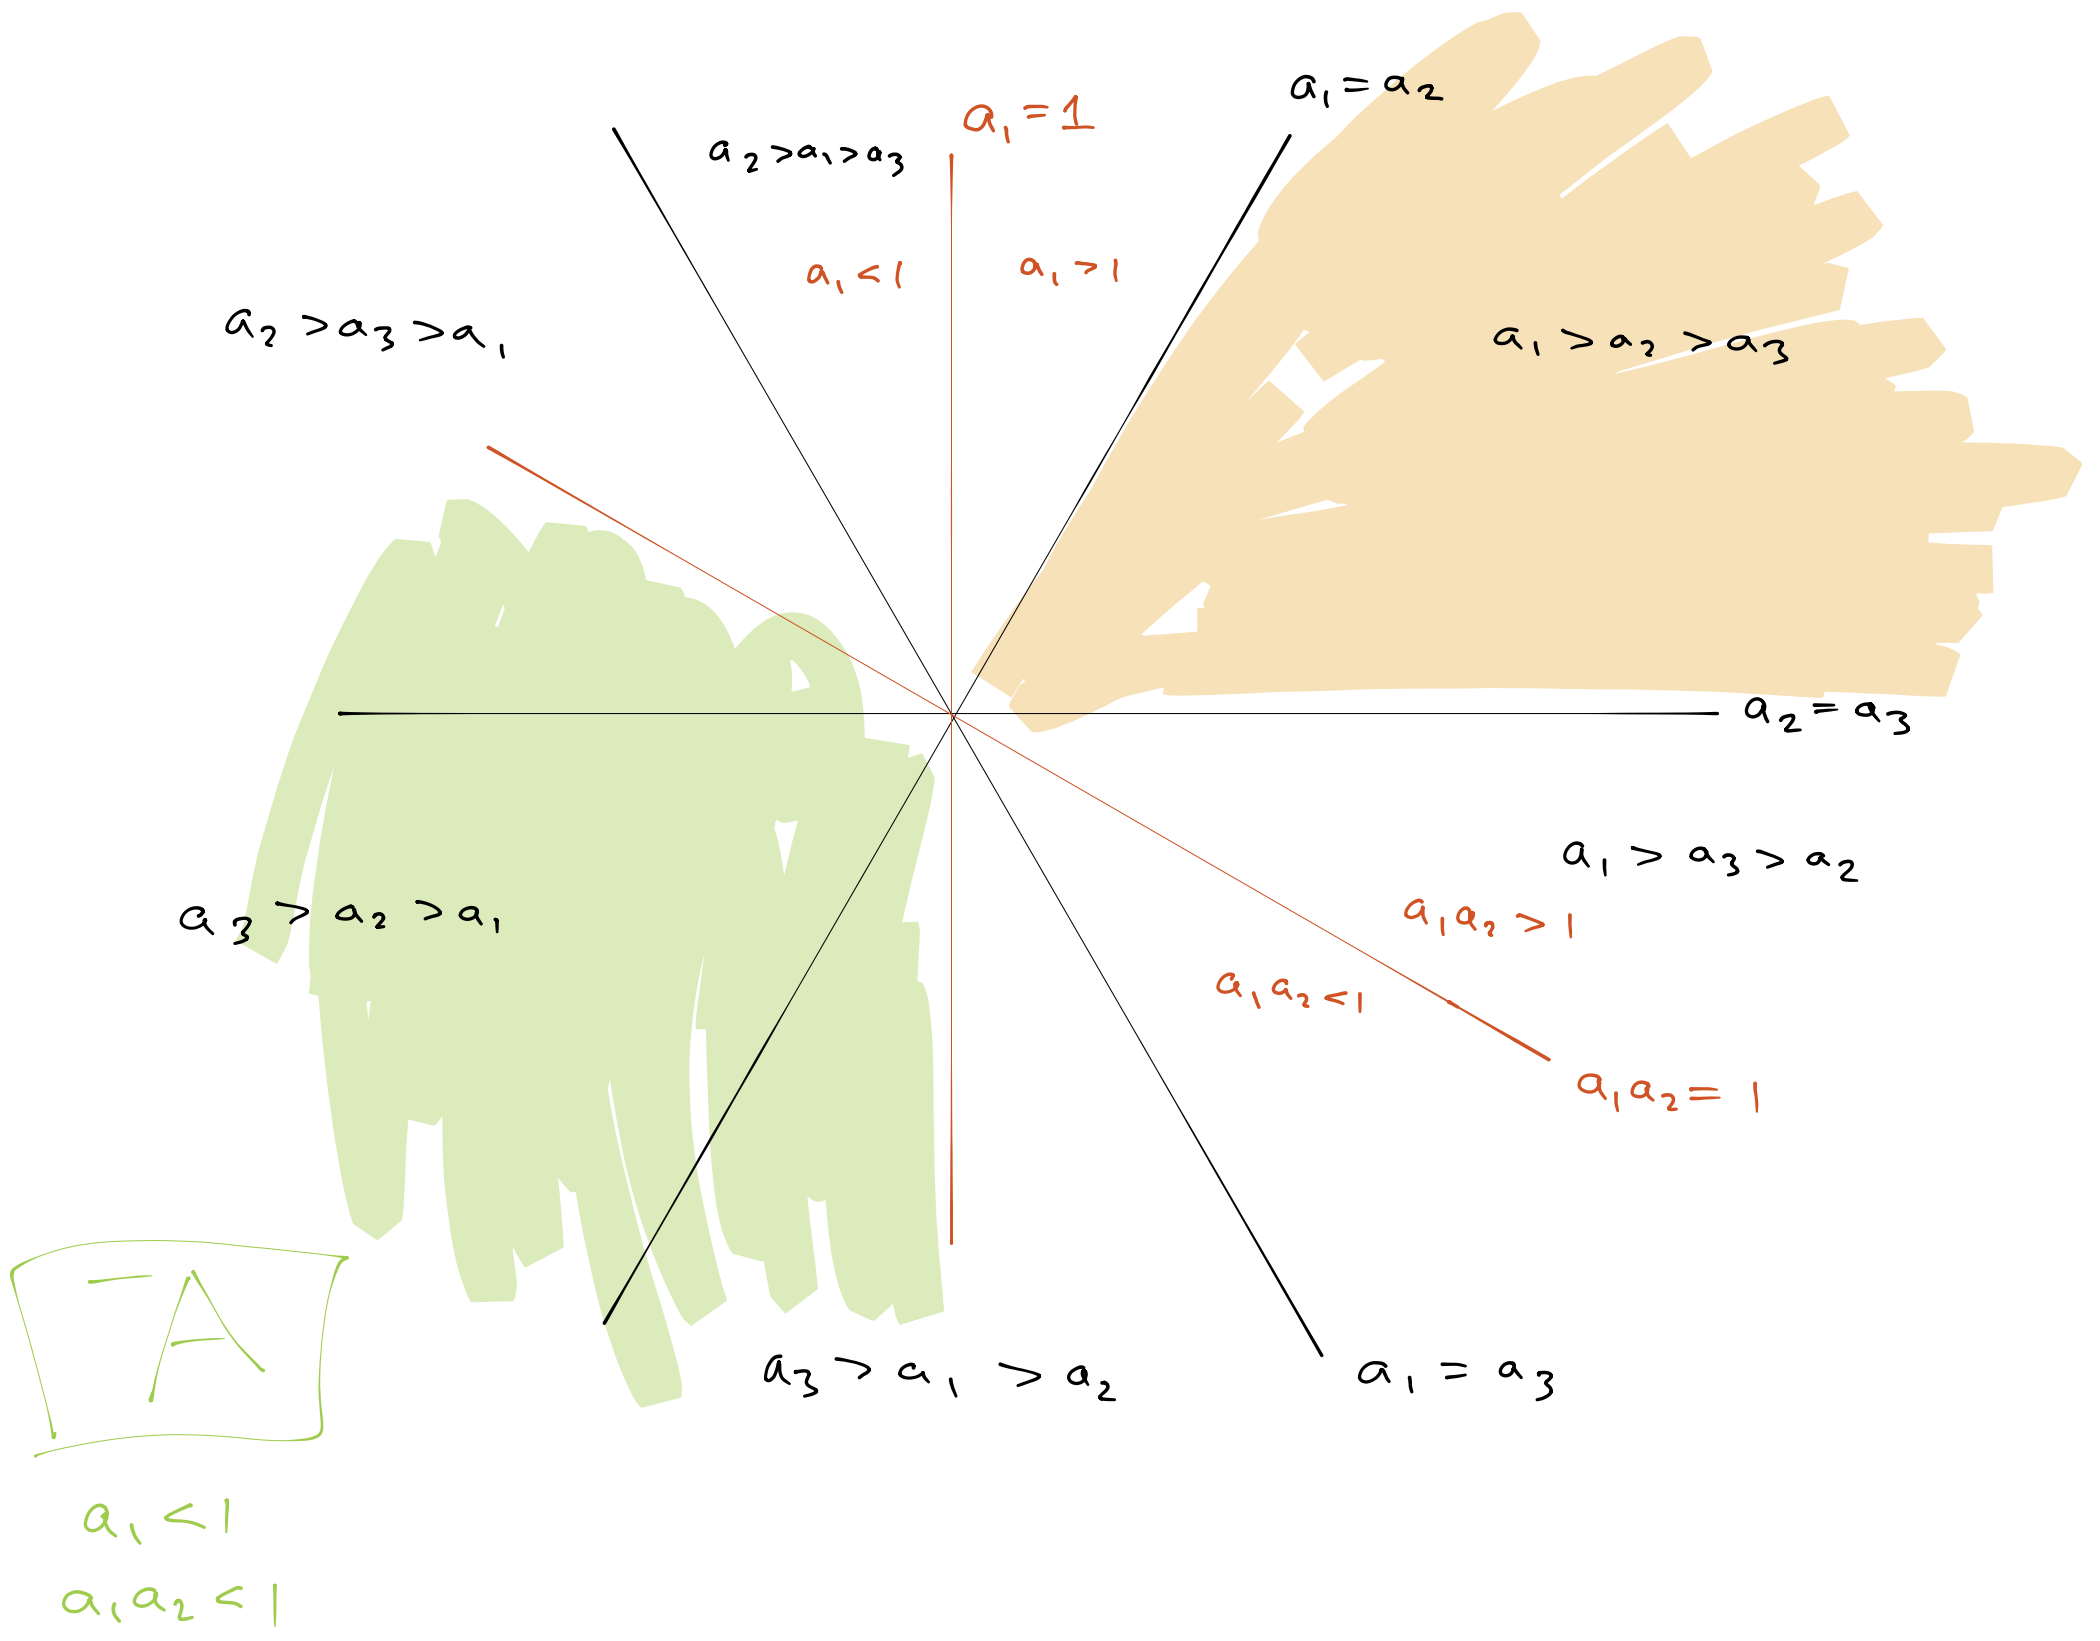
\includegraphics[width=12.8 cm, height = 10 cm]{map-A-SL3.png}
  \caption{ A ``map'' of the diagonal subgroup $A \leq \SL_3(\mathbb{R})$.  }
\end{figure}


One more easy lemma:
\begin{lemma}\label{lem:stoes2021:let-omega-be}
  Let $\Omega$ be a compact subset of $G$.  Then there is a compact subset $\Omega _A$ of $A$ so that $a(x g) \in a(x) \Omega_A$ for all $x \in G$ and $g \in \Omega$.
\end{lemma}
\begin{proof}
  By enlarging $\Omega$ if necessary, we may assume that it is closed under left and right multiplication by the compact subgroup $K$ of $G$.  Write $x = u a k$ (Iwasawa decomposition).  Then $x g = u a k g$ with $k g \in \Omega$.  By the Iwasawa decomposition, we may find a compact subset $\Omega_A \subseteq A$ so that $\Omega \subseteq N \Omega_A K$.  Then $k g$ admits the Iwasawa decomposition $u' a' k'$ with $a' \in \Omega_A$.  We have $x g = u (a u' a^{-1}) a a' k'$.  Since $A$ normalizes $N$, this shows that $a(x g) = a a' \in a \Omega_A$, as required.
\end{proof}

\subsubsection{Proof of Theorem \ref{thm:2}}
We must show that if $g$ belongs to a fixed compact subset of $G$ and $s$ belongs to a fixed compact subset of the region $\{s : s - 2 \rho \text{ strictly dominant}\}$, then $\sum _{\gamma \in \Gamma_B \backslash \Gamma } a(\gamma g)^s \ll 1$.

By Lemma \ref{lem:stoes2021:let-omega-be}, we have for $g$ and $s$ as above and all $\gamma \in \Gamma$ the estimate
\begin{equation*}
  a(\gamma g) ^s  \asymp a (\gamma) ^s
\end{equation*}
Moreover, if $s$ lies in $\mathbb{R}^n$, then each of the above quantities is positive.  The theorem will thus follow if we can show that for each $s \in \mathbb{R}^n $ with $s - 2 \rho $ strictly dominant,
\begin{equation*}
  \sum _{\gamma \in \Gamma_B \backslash \Gamma } a (\gamma ) ^s < \infty.
\end{equation*}

Since the subgroup $\Gamma$ of $G$ is discrete, we may find a nonempty bounded neighborhood $\Omega \subseteq G$ of the identity element such that the translates $\gamma \Omega$ for $\gamma \in \Gamma$ are disjoint from one another.  By another application of Lemma \ref{lem:stoes2021:let-omega-be}, we have
\begin{equation*}
  a(\gamma)^s \asymp a(\gamma g)^s
\end{equation*}
for all $\gamma \in \Gamma$ and $g \in \Omega$.  We thereby reduce to verifying that
\begin{equation*}
  \int _{g \in \Omega }\sum _{\gamma \in \Gamma_B \backslash \Gamma } a (\gamma g ) ^s \, d g < \infty.
\end{equation*}

The sets $\Gamma_B \gamma \Omega$ for coset representatives $\gamma \in \Gamma_B \backslash \Gamma$ are disjoint from one another, so it is enough to verify that
\begin{equation*}
  \int _{g \in \Gamma_B \backslash \Gamma \Omega} a (g) ^s \,d g < \infty ,
\end{equation*}
where now $d g$ denotes the quotient Haar measure on $\Gamma _B \backslash G$.

Let $\gamma \in \Gamma$ and $g \in \Omega$.  Let $\omega$ be a dominant weight.  By Lemma \ref{lem:stoes2021:let-omega-be}, we have $a(\gamma g)^{\omega} \ll a(\gamma)^{\omega} a(g)^{\omega}$.  Recalling from Lemma \ref{lem:stoes2021:each-dominant-weight} that $a(\gamma)^{\omega} \leq 1$ and from, e.g., Lemma \ref{lem:stoes2021:let-omega-be} that $a(\gamma)^{\omega} \ll 1$, we obtain
\begin{equation*}
  a(\gamma g)^{\omega} \ll 1.
\end{equation*}

This last estimate tells us that each $g \in \Gamma \Omega$ satisfies $a(g) \in c \cdot {}^- A$ for some fixed $c \in A$, depending at most upon $\Omega$.  In other words,
\begin{equation*}
  \Gamma \Omega \subseteq N \cdot c \cdot {}^- A \cdot K.
\end{equation*}
We thereby reduce to verifying that
\begin{equation*}
  \int _{g \in \Gamma_B \backslash N \cdot c \cdot {}^- A \cdot K} a(g)^s \, d g < \infty.
\end{equation*}

We now recall from Example \ref{exa:2} that a Haar measure $d g$ may be given in Iwasawa coordinates $g = u a k$ by $d u \, \frac{d a}{a^{2 \rho}} \, d k$.  The quotient $\Gamma_N \backslash N$ is compact because it is the image of the compact set $\{u \in N : |u_{i j}| \leq 1/2 \forall i < j\}$, as one verifies readily either directly or by adopting the proof of Theorem \ref{thm:existence-reduced-basis}.  The group $K$ is compact.  We thereby reduce to verifying the finiteness of
\begin{equation}
  \int _{a \in {}^- A}
  a^{s - 2 \rho}
  \, d a
\end{equation}
whenever $s - 2 \rho$ is strictly dominant, where as usual $d a$ denotes a Haar measure on $A$, e.g., that given by
\begin{equation*}
  d a = \frac{d a _1 \dotsb d a _{n - 1}}{a_1 \dotsb a_{n-1}}.
\end{equation*}

At this point, we might as well substitute $s \mapsto s + 2 \rho$ to reduce to verifying that
\begin{equation}\label{eq:int-_a-in}
  \int _{a \in {}^- A}
  a^{s}
  \, d a
\end{equation}
is finite whenever $s$ is strictly dominant.

To understand the last integral \eqref{eq:int-_a-in}, we change coordinates to
\begin{equation*}
  t_m = a_1 \dotsb a_m \quad (1 \leq m \leq n - 1 ).
\end{equation*}
In these coordinates, the domain ${}^- A$ is described by the conditions $t_m \leq 1$ for all $m$.  Moreover, if define $\nu_1, \dotsc, \nu_{n-1}$ by
\begin{equation*}
  \nu_m := s_m - s_{m+1} > 0,
\end{equation*}
then we have
\begin{equation*}
  s_m = \nu_m + \nu_{m+1} + \dotsb + \nu_{n-1} + s_n
\end{equation*}
and
\begin{equation*}
  a^s = \prod_{m=1}^{n-1} t_m^{\nu_m}.
\end{equation*}
The integral \eqref{eq:int-_a-in} of interest thus factors as the product of one-dimensional integrals
\begin{equation*}
  \int _{t_m = 0}^1 t_m^{\nu_m} \, \frac{d t_m}{t_m},
\end{equation*}
each of which converge.  The proof is thus complete.

\begin{exercise}
  For $\gamma \in \Gamma = \SL_n(\mathbb{Z})$, write $a_1(\gamma), \dotsc, a_n(\gamma) > 0$ for the Iwasawa coordinates.  Note that these depend only upon the coset $\Gamma_B \gamma$.  For $1 \leq m \leq n-1$, define $t_m(\gamma) := a_1(\gamma) a_2(\gamma) \dotsb a_m(\gamma)$.

  Show that for $X_1, \dotsc, X_{n-1} \geq 1$,
  \begin{equation*}
    \# \left\{ \gamma \in \Gamma_B \backslash \Gamma : t_m(\gamma) \geq 1/X_m \text{ for all } 1 \leq m \leq n-1 \right\} \ll (X_1 \dotsb X_{n-1})^2.
  \end{equation*}
  Show also that for $X \geq 1$,
  \begin{equation*}
    \# \left\{ \gamma \in \Gamma_B \backslash \Gamma : a_i(\gamma) / a_{i+1}(\gamma) \geq 1/X \text{ for all } 1 \leq i \leq n-1 \right\} \ll X^p
  \end{equation*}
  for some $p = p(n) > 0$.
\end{exercise}

\begin{exercise}
  Let $\mathfrak{S} \leq G$ be a Siegel domain, and $\Omega \subseteq G$ a compact subset.
  \begin{enumerate}
  \item Show that there exists $c \geq 1$ with the following property.  Let $x \in \mathfrak{S}$ and $\gamma \in \Gamma$.  Suppose that $\gamma x \in N x \Omega$.  Let $1 \leq i < j \leq n$ be indices such that the Iwasawa coordinates $a_1,\dotsc,a_n$ of $x$ satisfy $a_i / a_j \geq c$.  Then $\gamma_{j i} = 0$.
  \item Show that for each $g \in \mathfrak{S}$,
    \begin{equation*}
      \# \{ \gamma \in \Gamma : g^{-1} \gamma g \in \Omega \} \ll a(g)^{2 \rho}.
    \end{equation*}
  \item Show that there is a bounded subset of $\mathfrak{S}$ containing all $g \in \mathfrak{S}$
    for which $\gamma g \in N \Omega$ for some  $\gamma \in \Gamma$.
    % see log entry [[Eisenstein series attached to compactly-supported functions are compactly-supported]]
  \end{enumerate}
\end{exercise}


\section{Basics on automorphic forms}

At least initially, we'll follow in large part the exposition of Borel \cite[\S2]{MR2331343}.
\subsection{Motivation}
Sometimes it's useful to break problems up into analytic and algebraic parts.  For instance, as a first step towards the analysis of spaces of functions on the circle group $\mathbb{R} / \mathbb{Z}$, one can study the algebraically-flavored space of trigonometric polynomials, i.e., finite linear combinations of the functions $x \mapsto e(n x)$ ($n \in \mathbb{Z}$).  It's straightforward to verify that the Fourier inversion formula and the Parseval relation hold for such functions.  One can then deduce the corresponding assertions for more analytically-flavored spaces (e.g., the space $L^2(\mathbb{R}/\mathbb{Z})$ of square-integrable functions the space $C^\infty(\mathbb{R}/\mathbb{Z})$ of smooth functions, etc.) via limiting arguments.  Similarly, on the real line, one can approach analytic questions concerning function spaces ($L^2(\mathbb{R})$, the Schwartz space $\mathcal{S}(\mathbb{R})$, etc.) by first studying algebraic questions concerning finite linear combinations of Fourier modes $x \mapsto e(\xi x)$ ($\xi \in \mathbb{R}$), or finite linear combinations of hermite functions, i.e., functions of the form $x \mapsto P(x) e^{- \pi x^2}$ for a polynomial $P$.

Automorphic forms are algebraically-flavored spaces of functions on $\Gamma \backslash G$.

\subsection{Definition without explanation}\label{sec:defin-with-expl}
We continue to focus on the examples $\Gamma \backslash G = \SL_n (\mathbb{Z}) \backslash \SL_n(\mathbb{R})$ or $\GL_n(\mathbb{Z}) \backslash \GL_n(\mathbb{R})$.  We accordingly let $K$ denote $\SO(n)$ or $\O(n)$.

\begin{definition}\label{defn:an-emph-form}
  An \emph{automorphic form} $\varphi : G \rightarrow \mathbb{C}$ is a continuous function such that
  \begin{enumerate}
  \item [($A_1$)] $\varphi(\gamma x) = \varphi (x)$ for all $\gamma \in \Gamma$, $x \in G$
  \item [($A_2$)] $\varphi$ is \emph{right $K$-finite}, i.e., the span of $\{\varphi(\cdot k) : k \in K\}$ is finite-dimensional.
  \item [($A_3$)] $\varphi$ is \emph{$\mathfrak{Z}(\mathfrak{g})$-finite}, where $\mathfrak{Z}(\mathfrak{g})$ denotes the center of the universal enveloping algebra.
  \item [($A_4$)] $\varphi$ is of \emph{moderate growth}.
  \end{enumerate}
\end{definition}
The conditions in this definition are elaborated below.

\subsection{Norms on $G$}
For $x \in G$, we define
\begin{equation*}
  \|x\|^2 := \sum _{i, j } \left(|x_{i j}|^2 + |(x^{-1})_{i j}|^2\right).
\end{equation*}
We observe that
\begin{equation*}
  \|x y\| \leq \|x\| . \|y\|, \quad \|x\| = \|x^{-1}\|,
\end{equation*}
that $\{x \in G : \|x\| \leq c\}$ is compact for each $c > 0$, and that for each compact subset $\Omega$ of $G$,
\begin{equation}\label{eq:u-x-u}
  \|u x u'\| \asymp \|x\| \quad (u, u' \in \Omega, x \in G).
\end{equation}

\begin{exercise}
  Let $\mathfrak{S} \subseteq G = \SL_n(\mathbb{R})$ be a Siegel domain (Definition \ref{defn:siegel-domain}).
  Let $\omega$ be a dominant weight (\S\ref{sec:recap-finite-dimens}).
  Show that there exists $m > 0$ such that for each compact subset $\Omega \subseteq G$ there exists $C$ so that for all $\gamma \in \Gamma$, $x \in \mathfrak{S}$ and $g \in \Omega$,
  \begin{equation*}
    a(x)^{\omega} \leq C \|\gamma x g\|^m.
  \end{equation*}
  [Hint: use that $\|h\| \asymp \|h g\|$ for $g \in \Omega$ and that if $x \in B$, then $a(x)^{\omega} = \|x e_\omega \|$.]
\end{exercise}


\subsection{Functions of moderate growth}\label{sec:funct-moder-growth}
We say that a function $f : G \rightarrow \mathbb{C}$ is of \emph{moderate growth} if there exists $m \in \mathbb{Z}$ so that
\begin{equation}\label{eq:fx-ll-xm}
  f(x) \ll \|x\|^m
  \quad (x \in G).
\end{equation}
We say that $f$ is of \emph{rapid decay} if the estimate \eqref{eq:fx-ll-xm} holds for all $m \in \mathbb{Z}$.

It is clear that a sum or product of functions of moderate growth or rapid decay has the same property, while the product of one function of moderate growth with another function of rapid decay is of rapid decay.  Thus the functions of moderate growth form a ring which contains the functions of rapid decay as an ideal.


\subsection{Finite functions}

\subsubsection{Generalities}


\begin{lemma}
  Let $G$ be a locally compact group.  Let $f : G \rightarrow \mathbb{C}$ be a continuous function (measurability would also suffice).  The following conditions are equivalent:
  \begin{enumerate}
    [(i)]
  \item The span of the right $G$-translates of $f$ is finite-dimensional.
  \item The span of the left $G$-translates of $f$ is finite-dimensional.
  \item The span of the $G \times G$-translates of $f$ is finite-dimensional.
  \item $f$ arises as a matrix coefficient for some finite-dimensional representation $(\pi,V)$ of $G$: there exists $\alpha \in \End(V)^*$ so that $f(g) = \alpha(\pi(g))$.
  \end{enumerate}
\end{lemma}
\begin{definition}
  A \emph{finite function} on $G$ is one satisfying the equivalent conditions of the lemma.
\end{definition}

\begin{example}
  For $G = \mathbb{R} = \mathbb{R} / \mathbb{Z}$, the finite functions are the trigonometric polynomials, i.e., the finite linear combinations of $x \mapsto e(n x)$.
\end{example}

\begin{example}
  For a compact group $G$, any finite-dimensional representation decomposes as a direct sum of irreducible representations, so the finite functions are the finite linear combinations of matrix coefficients of irreducible finite-dimensional representations.  The Peter--Weyl theorem says that these are dense in $L^2(G)$.
\end{example}

\begin{example}
  For $G = \mathbb{R}$, the finite functions are the finite linear combinations of the \emph{exponential polynomials}
  \begin{equation*}
    x \mapsto e^{\alpha x} x^{\beta}
  \end{equation*}
  defined for $\alpha \in \mathbb{C}$ and $\beta \in \mathbb{Z}_{\geq 0}$.

  These are also the generalized eigenfunctions of the differentiation operator $\partial_x = \frac{d}{d x}$, i.e., the function $f$ for which $(\partial_x - \alpha )^{\beta+1} f = 0$.
\end{example}
\begin{example}\label{exa:g-=-mathbbrtimes_+}
  For $G = \mathbb{R}^\times_+ \xrightarrow{\log} \mathbb{R}$, the finite functions are those of the form
  \begin{equation*}
    y \mapsto y^{\alpha} (\log y)^{\beta},
  \end{equation*}
  with $\alpha$ and $\beta$ as above.  These are also called exponential polynomials.
\end{example}

\subsubsection{Isotypic decomposition}\label{sec:isotyp-decomp}
Let $K$ and $G$ be as in Definition \ref{defn:an-emph-form}.  Let $\varphi : G \rightarrow \mathbb{C}$ be a right $K$-finite continuous function.  Write $V$ for the (finite-dimensional) span of the right translates of $\varphi$.  Then $K$ acts on $V$ via right translation.  By Maschke's theorem, we may decompose $V$ as a direct sum of irreducible representations of $K$.

Let $\sigma$ be an irreducible representation of $K$.  We say that $\varphi$ has \emph{$K$-type $\sigma$} if $V$ is isomorphic to a direct sum of copies of $\sigma$. Define $e_\sigma \in C^\infty(K)$ by the formula
\begin{equation*}
  e_\sigma(k) := (\dim \sigma) \chi_\sigma(k),
\end{equation*}
where $\chi_\sigma(k) := \trace(\sigma(k))$ denotes the character of $\sigma$.  Using the Schur orthogonality relations, we may check that $\varphi$ has $K$-type $\sigma$ if and only if the convolution
\begin{equation*}
  \varphi \ast e_\sigma : g \mapsto \int_{k \in K} \varphi(g k^{-1}) e_\sigma(k) \, d k,
\end{equation*}
defined using the probability Haar measure $d k$ on $K$, coincides with $\varphi$, i.e., $\varphi \ast e _\sigma = \varphi$.

We say that $V$ is \emph{$K$-isotypic} if it has $K$-type $\sigma$ for some $\sigma$.  In general, we may write any $K$-finite $\varphi$ as a finite sum of $K$-isotypic vectors, indexed by $\sigma$ in some finite collection $\Xi$ of (isomorphism classes of) irreducible representations of $K$.  For any such $\Xi$, set
\begin{equation*}
  e _{\Xi } := \sum _{\sigma \in \Xi } e _\sigma.
\end{equation*}
Then a continuous function $\varphi$ on $G$ is $K$-finite if and only if it satisfies $\varphi \ast e _{\Xi } = \varphi$ for some such $\Xi$.

\subsection{Universal enveloping algebra}\label{sec:univ-envel-algebra}

\subsubsection{General definition and construction}\label{sec:gener-defin-constr}

Let $\mathfrak{g}$ be a Lie algebra.
\begin{definition}
  A \emph{universal enveloping algebra} $\mathfrak{U}(\mathfrak{g})$ is a unital associative algebra equipped with a morphism of Lie algebras $\mathfrak{g} \rightarrow \mathfrak{U}(\mathfrak{g})$ that is universal among such morphisms in the following sense: for each morphism of Lie algebras $\mathfrak{g} \rightarrow A$ whose target is unital associative algebra $A$, there is a unique morphism of associative algebras $\mathfrak{U}(\mathfrak{g}) \rightarrow A$ such that the composition $\mathfrak{g} \rightarrow \mathfrak{U}(\mathfrak{g}) \rightarrow A$ is the given map $\mathfrak{g} \rightarrow A$.
\end{definition}
By the usual arguments, if such an algebra exists, then it is unique.  For this reason we typically speak of ``the'' universal enveloping algebra.  We may construct $\mathfrak{U}(\mathfrak{g})$ explicitly as the quotient $T(\mathfrak{g})/I$, where
\begin{itemize}
\item $T(\mathfrak{g})$ denotes the tensor algebra of $\mathfrak{g}$, i.e., the graded algebra $\oplus_{k \in \mathbb{Z}_{\geq 0}} \mathfrak{g}^{\otimes k}$ equipped with the multiplication
  \begin{equation*}
    (x_1 \otimes \dotsb \otimes x_{k_1}) \cdot (y_1 \otimes \dotsb \otimes y_{k_2}) = x_1 \otimes \dotsb \otimes x_{k_1} \otimes y_1 \otimes \dotsb \otimes y_{k_2},
  \end{equation*}
  and
\item $I$ denotes the ideal of $T(\mathfrak{g})$ generated by the elements $x \otimes y - y \otimes x - [x,y]$ for $x, y \in \mathfrak{g}$.
\end{itemize}
In other words, $\mathfrak{U}(\mathfrak{g})$ may be regarded as the non-commutative polynomial ring generated by elements $X \in \mathfrak{g}$ subject to the relations $X Y - Y X = [X,Y]$.

The proof that this construction defines a universal enveloping algebra is the same as the proof that, e.g., the usual construction of the tensor product of a pair of vector spaces satisfies its universal property.

\subsubsection{Construction via Lie theory}\label{sec:construction-via-lie}
Let $G$ be a Lie group.  We'll assume that it's a closed subgroup of $\GL_n(\mathbb{R})$.  Then $\mathfrak{g} := \Lie(\mathfrak{g})$ may be identified with a Lie subalgebra of the algebra $M_n(\mathbb{R})$ of $n \times n$ matrices.

The group $G$ acts on itself by left and right translation, hence also on functions on $G$.  For $g \in G$ and $f : G \rightarrow \mathbb{C}$, we set
\begin{equation*}
  r_g f(x) := f(x g), \quad \ell_g f(x) := f(g^{-1} x).
\end{equation*}
These define the right and left regular representations of $G$.
\begin{exercise}
  Verify that $r_{g_1} r_{g_2} = r_{g_1 g_2}$ and $\ell_{g_1} \ell_{g_2} = \ell_{g_1 g_2}$.
\end{exercise}

For $X \in \mathfrak{g}$, we write $e^X = \exp(X) \in G$ for its exponential, which may be defined by the usual series.  Thus
\begin{equation*}
  e^{t X} = \sum _{n \geq 0} \frac{t^n X^n}{n!}.
\end{equation*}

The group $G$ acts on itself by conjugation.  This induces the adjoint representation of $G$ on $\mathfrak{g}$, denoted $\Ad : G \rightarrow \GL(\mathfrak{g})$.  We have
\begin{equation*}
  g e^{t X} g^{-1} = e^{t \Ad(g) X}.
\end{equation*}

Each $X \in \mathfrak{g}$ defines a left-invariant differential operator on $G$, i.e., an element $[f \mapsto X f]$ of $\End(C^\infty(G))$ given by
\begin{equation*}
  X f(g) := \partial_{t=0} f(g e^{t X}).
\end{equation*}
In other words, $X f = \partial_{t=0} r_{e^{t X}} f$ is obtained by differentiating the right regular representation of $G$.  The Lie bracket $[,]$ on $\mathfrak{g}$ is characterized by the identity
\begin{equation}\label{eq:x-y-f}
  X (Y  f) - Y (X f) = [X,Y] f
  \quad (f \in C^\infty(G)).
\end{equation}
The map $\mathfrak{g} \rightarrow \End(C^\infty(G))$ is thus a Lie algebra homomorphism.  This map is readily seen to be injective (consider the first order Taylor coefficients of $f$ at the identity), so we may identify $\mathfrak{g}$ with its image.

The universal enveloping algebra $\mathcal{U}(\mathfrak{g})$ may be defined as the subalgebra of $\End(C^\infty(G))$ generated by $\mathfrak{g}$.  (It is clear from the universal propetry that $\mathfrak{U}(\mathfrak{g})$, as constructed in \S\ref{sec:gener-defin-constr}, admits a map to $\End(C^\infty(G))$.  The point is just that this map is injective.)  We may also identify $\mathcal{U}(\mathfrak{g})$ with the algebra of left-invariant differential operators on $G$, or with the convolution algebra of distributions on $G$ supported at the identity element.

\subsubsection{The center}

\begin{definition}
  We denote by $\mathfrak{Z}(\mathfrak{g})$ the center of $\mathfrak{U}(\mathfrak{g})$.
\end{definition}

\begin{definition}
  In the setting of \S\ref{sec:defin-with-expl}, we say that $\varphi : G \rightarrow \mathbb{C}$ is \emph{$\mathfrak{Z}(\mathfrak{g})$-finite} if the image of its span under the action of $\mathfrak{Z}(\mathfrak{g})$ described in \S \ref{sec:construction-via-lie} is finite-dimensional.
\end{definition}

\begin{example}\label{example:stoes2021:g-=-gl_nmathbbr}
  For $G = \GL_n(\mathbb{R})$, $\mathfrak{Z}(\mathfrak{g})$ is isomorphic to a polynomial ring in $n$ variables, described explicitly via the Harish--Chandra isomorphism \cite[p.220]{MR855239}.
\end{example}

\begin{example}\label{exa:g-=-sl_2mathbbr}
  For $G = \SL_2(\mathbb{R})$, $\mathfrak{Z}(\mathfrak{g})$ is isomorphic to a polynomial ring in one variable.  It is freely generated by the element
  \begin{equation}\label{eq:omega-=-e}
    \Omega
    = e f + f e + \frac{1}{2} h ^2,
  \end{equation}
  where
  \begin{equation*}
    e = 
    \begin{pmatrix}
      0 & 1 \\
      0 & 0
    \end{pmatrix}
    , \quad f = 
    \begin{pmatrix}
      0 & 0 \\
      1 & 0
    \end{pmatrix}
    , \quad h = 
    \begin{pmatrix}
      1 & 0 \\
      0 & -1
    \end{pmatrix}
    .
  \end{equation*}
  This is the simplest example of a ``Casimir element.''  Note that in \eqref{eq:omega-=-e}, the products $ef, f e, h^2$ take place inside $\mathfrak{U}(\mathfrak{g})$, not inside the space of $2 \times 2$ matrices.
\end{example}

\subsection{Finiteness}\label{sec:Z-g-finiteness}
The algebra $\mathfrak{Z}(\mathfrak{g})$ acts on the space of smooth functions $\varphi$ on $G$ (and also on, e.g., the space of distributions).  The space $\mathfrak{Z}(\mathfrak{g}) \varphi = \{D \varphi : D \in \mathfrak{Z}(\mathfrak{g})\}$ is isomorphic to the quotient algebra $\mathfrak{Z}(\mathfrak{g}) / \Ann(\varphi)$, where $\Ann(\varphi) = \{D : D \varphi = 0\}$ denotes the annihilator ideal of $\varphi$.  Thus that space is finite-dimensional if and only if that ideal is of finite codimension.  In particular, $\varphi$ is $\mathfrak{Z}(\mathfrak{g})$-finite if and only if it is annihilated by some ideal $J$ in $\mathfrak{Z}(\mathfrak{g})$ of finite codimension.  We say in the latter case that $\varphi$ has \emph{$\mathfrak{Z}(\mathfrak{g})$-type $J$}.

\subsection{Relation to classical modular forms}\label{sec:relat-class-modul}
Take $\Gamma \backslash G = \SL_2(\mathbb{Z}) \backslash \SL_2(\mathbb{R})$, $K = \SO(2)$.  Then $G/K$ identifies with the upper half-plane $\mathbb{H} = \{x + i y : y > 0\}$ via the map $g K \mapsto g \cdot i$, where $G$ acts on $\mathbb{H}$ via fractional linear transformations:
\begin{equation*}
  \begin{pmatrix}
    a & b \\
    c & d
  \end{pmatrix}
  \cdot z = \frac{a z + b }{c z + d}.
\end{equation*}
\begin{definition}\label{defn:function-f-:}
  A function $f : \mathbb{H} \rightarrow \mathbb{C}$ is a \emph{modular form of weight $m$} if
  \begin{enumerate}
  \item [($M_1$)] $f (\gamma z) = (c z + d) ^m f (z)$ for all $\gamma = 
    \begin{pmatrix}
      a & b \\
      c & d
    \end{pmatrix}
    \in \Gamma$ and $z \in \mathbb{H} $.
  \item [($M_2$)] $f$ is holomorphic.
  \item [($M_3$)] $f$ is ``regular at the cusp.''
  \end{enumerate}
\end{definition}
Explanation of ($M_3$): from ($M_1$) we see that $f(z+1) = f(z)$, then from ($M _2 $) that $f(z) = \sum _{n \in \mathbb{Z} } a_n e(n z)$, where as usual $e(z) := e^{2 \pi i z}$.  The factor $e (n z)$ blows up as $y \rightarrow \infty$ if $n < 0$.  Condition ($M_3$) says that $a_n = 0$ unless $n \geq 0$, so that such blow-up does not occur.

The relation between Definition \ref{defn:function-f-:} and Definition \ref{defn:an-emph-form} is as follows.  Given a modular form $f$ of weight $m$, define a function $\varphi : G \rightarrow \mathbb{C} $ by
\begin{equation*}
  \varphi (g) := (c i + d)^{-m} f (g \cdot i) \quad \text{ if } g = 
  \begin{pmatrix}
    a & b \\
    c & d
  \end{pmatrix}
  .
\end{equation*}
\begin{exercise}
  Show that ($M_1$) implies ($A_1$).
\end{exercise}
\begin{exercise}
  Show that ($M_1$) implies ($A_2$); more precisely, verify that
  \begin{equation*}
    \varphi \left( g 
      \begin{pmatrix}
        \cos \theta  & \sin \theta  \\
        -\sin \theta & \cos \theta
      \end{pmatrix}
    \right) = e (m \theta ) \varphi (\gamma).
  \end{equation*}
\end{exercise}
\begin{exercise}
  Show that ($M_2$) implies ($A_3$); more precisely, with $\Omega$ as in Example \ref{exa:g-=-sl_2mathbbr}, verify that $\Omega \varphi = c \varphi$ for some real number $c$ depending only upon $m$.
\end{exercise}
\begin{exercise}
  Show that ($M_3$) implies ($A_4$).
\end{exercise}

\begin{exercise}\label{exe:let-f-:}
  Let $f : \mathbb{H} \rightarrow \mathbb{C}$ be a smooth function on the upper half-plane that is an eigenfunction for the hyperbolic Laplacian $\Delta = y^2 (\partial_{x x} + \partial_{y y})$.  Define $\varphi$ as above, taking $m = 0$.  Verify that ($A_3$) holds for $\varphi$; more precisely, show that $\varphi$ is an eigenfunction for $\Omega$, with eigenvalue deterimined by that for $f$ with respect to $\Lambda$.
\end{exercise}

\subsection{Some basic properties}

Recall that a Lie group $G$ comes with natural analytic charts, given by local exponential coordinates.  We state here, without proof, some basic consequences of Definition \ref{defn:an-emph-form}.

Let $G = \SL_n(\mathbb{R})$ or $\GL_n(\mathbb{R})$.
\begin{theorem}
  Any automorphic form is analytic.
\end{theorem}
More generally, any function $G \rightarrow \mathbb{C}$ that is right $K$-finite and $\mathfrak{Z}(\mathfrak{g})$-finite is analytic.  The idea of the proof is that the $K$-finiteness and $\mathfrak{Z}(\mathfrak{g})$-finiteness conditions imply that $\varphi$ satisfies an elliptic PDE.  See for instance \cite[Theorem 2.13]{MR1482800} or \cite[\S3.1]{MR2331343}.

\begin{theorem}[Harish--Chandra]\label{thm:harish-chandra-existence-reproducing-kernels}
  For any automorphic form $\varphi$ we may find $f \in C_c^\infty(G)$, supported arbitrarily close to the identity element, so that $\varphi$ equals the convolution $\varphi \ast f$ defined as usual by
  \begin{equation*}
    \varphi \ast f(x) := \int _{g \in G} \varphi(x g^{-1}) f(g) \, d g.
  \end{equation*}
  We may arrange moreover that $f(k^{-1} g k) = f(g)$ for all $k \in K, g \in G$.
\end{theorem}
This result again applies more generally to any right $K$-finite and $\mathfrak{Z}(\mathfrak{g})$-finite function on $G$.  See for instance \cite[Theorem 2.14]{MR1482800}, which develops a detailed proof in the special case $G = \SL_2(\mathbb{R})$, and \cite[Corollary 8.41]{MR855239} or \cite[\S3.2]{MR2331343} concerning the general case.

\begin{exercise}
  Assuming the statement of \cite[Theorem 1.14]{MR1942691}, deduce the conclusion of Theorem \ref{thm:harish-chandra-existence-reproducing-kernels} in the setting of Exercise \ref{exe:let-f-:}.
\end{exercise}

\begin{definition}\label{defn:we-say-that-uniform-moderate-growth}
  We say that a function $\varphi : G \rightarrow \mathbb{C}$ has \emph{uniform moderate growth} if there exists $m$ so that for each $D \in \mathcal{U}(\mathfrak{g})$, the function $D f$, defined as in \S\ref{sec:construction-via-lie}, satisfies \eqref{eq:fx-ll-xm}.
\end{definition}

\begin{proposition}
  Any automorphic form $\varphi$ has uniform moderate growth.
\end{proposition}
\begin{proof}
  Write $\varphi = \varphi \ast f$ with $f \in C_c^\infty(G)$.
  By elementary calculations with the definitions,
  we verify that
  \begin{equation*}
    D \varphi = D (\varphi \ast f) = \varphi \ast D f.
  \end{equation*}
  On the other hand, using \eqref{eq:u-x-u},
  we see that
  \begin{equation*}
    \varphi(g) \ll \|g\|^m
    \implies
    (\varphi \ast D f) \ll \|g\|^m.
  \end{equation*}
  Therefore $D \varphi(g) \ll \|g\|^m$, as required.
\end{proof}

\section{Constant terms}
The main purpose of this section is to generalize the basic estimate
\begin{equation}\label{eq:sum_n-geq-0}
  \sum_{n \geq 0} a_n e^{2 \pi i n z} \sim a_0
\end{equation}
describing the asymptotic behavior as $y \rightarrow \infty$ of classical modular forms.  More precisely, we initiate the study of the asymptotics ``near infinity'' in $\Gamma \backslash G$ of an automorphic form.  In this section $\Gamma \backslash G$ is either $\SL_n(\mathbb{Z}) \backslash \SL_n(\mathbb{R})$ or $\GL_n(\mathbb{Z}) \backslash \GL_n(\mathbb{R})$.  We loosely follow the exposition of \cite[\S5--6]{MR2331343}.

\subsection{Reduction from $\GL_n$ to $\SL_n$}\label{sec:reduction-from-gl_n}
Recall from Example \ref{exa:g-=-mathbbrtimes_+} that the finite functions on $\mathbb{R}^\times_+$ are the exponential polynomials.  The finite functions on $\mathbb{R}^\times$ will also be referred to as exponential polynomials (they are given on each of the two connected components by an exponential polynomial).

Take $G := \GL_n(\mathbb{R})$.  We may identify the center $Z$ of $G$ with $\mathbb{R}^\times$ via the map
\begin{equation*}
  \begin{pmatrix}
    z &  &  &  &  \\
      & z &  &  &  \\
      &  & \ddots &  &  \\
      &  &  & z &  \\
      &  &  &  & z
  \end{pmatrix}
  \mapsto z.
\end{equation*}
Using that $G$ commutes with $Z$, we deduce that the Lie algebra $\mathfrak{z}$ of $Z$, regarded as a subspace of the universal enveloping algebra $\mathfrak{U}(\mathfrak{g})$, lies in the center $\mathfrak{Z}(\mathfrak{g})$.  Thus any automorphic form $\varphi$ on $\Gamma \backslash G$ is in particular $\mathfrak{z}$-finite.  By analyticity, it is also $Z$-finite.  Therefore for each $g \in G$, the function $Z \ni z \mapsto \varphi(z g)$ is an exponential polynomial.  We get a slightly stronger conclusion by taking into account also the $\mathfrak{Z}(\mathfrak{g})$-finiteness of $\varphi$ (see \cite[\S5.6]{MR2331343} and references):
\begin{lemma}
  For each smooth $\mathfrak{Z}(\mathfrak{g})$-finite function $\varphi : G \rightarrow \mathbb{C}$,
  there are exponential polynomials $Q_i $ on $Z$
  and elements $P_i \in \mathfrak{Z}(\mathfrak{g})$ such that for all $z \in Z$ and $g \in G$, we have
  \begin{equation}
    \varphi (z g) = \sum _{i} Q_i(z) \cdot P_i f(g),
  \end{equation}
  with $P_i f$ defined as in \S\ref{sec:construction-via-lie}.
\end{lemma}

Since the multiplication map $Z \times \SL_n(\mathbb{R}) \rightarrow \GL_n(\mathbb{R})$ has image of finite index and since exponential polynomials may be regarded as well-understood, we see that the study of the behavior near infinity of automorphic forms on $\GL_n(\mathbb{Z}) \backslash \GL_n(\mathbb{R})$ largely reduces to that of automorphic forms on $\SL_n(\mathbb{Z}) \backslash \SL_n(\mathbb{R})$.

\subsection{Standard parabolic subgroups}\label{sec:stand-parab-subgr}

Fix a Siegel domain $\mathfrak{S}$ for $\Gamma \backslash G$ (\S\ref{sec:org0d39d27}).
\begin{question}
  How can a sequence $x^{(\ell)} \in \mathfrak{S}$ ($\ell=1,2,3,\dotsc$) tend off to $\infty$?
\end{question}
Recall that we may write $x^{(\ell)} = u^{(\ell)} a^{(\ell)} k^{(\ell)}$, where $u^{(\ell)}$ lies in some fixed compact subset of $N$, $k^{(\ell)}$ lies in $K$, and $a^{(\ell)}$ is a diagonal matrix with positive entries for which each ratio $a_i^{(\ell)} / a_{i+1}^{(\ell)}$ is bounded from below by some fixed positive quantity.  Thus after passing to a subsequence, we may assume that each such ratio either remains bounded or tends off to infinity as $\ell \rightarrow \infty$.  Let $I \subseteq \{1, \dotsc, n-1\}$ denote the set of indices for which the ratio in question remains bounded.  Then $I$ describes the ``directions'' in which $x^{(\ell)}$ remains bounded in $\mathfrak{S}$, while the complement of $I$ describes those in which it tends off to infinity.

It is often convenient to think of the set $I$ in terms of a related equivalence relation $\sim$ on $\{1,\dotsc,n\}$.  We declare $i \sim j$ when the ratio $a_i^{(\ell)} / a_j^{(\ell)}$ is bounded from above and below by fixed positive quantities, independent of $\ell$.  Thus for $i \leq j$, we have $i \sim j$ precisely when $\{i,i+1,\dotsc,j-1\} \subseteq I$.  Such equivalence relations have the property that their equivalence classes consist of intervals of integers.  Let us call such relations \emph{continguous}.  We obtain a natural bijection
\begin{equation*}
  \{\text{subsets } I \subseteq \{1,\dotsc,n-1\}\}
  \leftrightarrow
  \{\text{contiguous equivalence relations $\sim$ on } \{1,\dotsc,n \}\}.
\end{equation*}
We may, in turn, identify a continguous equivalence relation with the
\emph{composition} of $n$ describing the cardinalities of each equivalence class.  For instance, if $n = 8$ and $I = \{1,3,4,7\}$, then the equivalence classes of $\sim$ are $\{1,2\}$, $\{3,4,5\}$,  $\{6\}$ and $\{7,8\}$, and the corresponding composition is $n = 2 + 3 + 1 + 2$.

(In the lecture, the following definition was given a bit later, when it seemed better motivated.)
\begin{definition}
  Given an equivalence relation $\sim$ on $\{1, \dotsc, n\}$ (or equivalently, a subset of $\{1, \dotsc, n-1\}$, or a composition of $n$), the corresponding \emph{standard parabolic subgroup} $P$ of $G$ is defined by
  \begin{equation*}
    P := \{g \in G : g_{i j} = 0 \text{ if } i > j \text{ and } i \not \sim j \}.
  \end{equation*}
  The corresponding \emph{standard Levi subgroup} $M$ of $P$ is defined by
  \begin{equation*}
    M := \{g \in G : g_{i j} = 0 \text{ if } i \not \sim j\}.
  \end{equation*}
  The \emph{unipotent radical} $U$ of $P$ is given by
  \begin{equation*}
    U := \{g \in N : g_{i j}  = 0 \text{ if } i \sim j\}.
  \end{equation*}
\end{definition}
Such subgroups have already appeared implicitly: in our discussion of the shape of Siegel domains (see handwritten notes from Lecture 2) and in our proof of Theorem \ref{thm:existence-reduced-basis}, part \eqref{item:siegel-finitely-many-gamma}.

\begin{exercise}
  With notation as above, we have $P = M U$.  More precisely, $P$ is the semidirect product of $M$ and $U$, with $U$ normal.
\end{exercise}


\begin{example}\label{example:stoes2021:take-g-=}
  Take $G = \SL_4$.  Given a sequence $x^{(\ell)}$, we get an equivalence relation $\sim$ (equivalently, a subset of $\{0,1,2,3\}$, or a composition of $4$), hence a standard parabolic subgroup $P = M U$.
  \begin{enumerate}
    [(i)]
  \item If $x^{(\ell)} = \diag(\ell^2, \ell, \ell^{-1}, \ell^{-2})$, then
    \begin{equation*}
      P = 
      \begin{pmatrix}
        \ast & \ast & \ast & \ast \\
             & \ast & \ast & \ast \\
             &  & \ast & \ast \\
             & & & \ast
      \end{pmatrix}
      , \quad M =
      \begin{pmatrix}
        \ast &  &  &  \\
             & \ast &  &  \\
             &  & \ast &  \\
             & & & \ast
      \end{pmatrix}
      , \quad U = 
      \begin{pmatrix}
        1 & \ast & \ast & \ast \\
          & 1 & \ast & \ast \\
          &  & 1 & \ast \\
          & & & 1
      \end{pmatrix}
      .
    \end{equation*}
    The corresponding subset and composition are
    \begin{equation*}
      \emptyset \subseteq \{0,1,2,3\},
      \quad
      4 = 1 + 1 + 1 +1.
    \end{equation*}
  \item If $x^{(\ell)} := \diag(\ell^2, \ell^2, \ell^{-1}, \ell^{-3})$, then
    \begin{equation*}
      P = 
      \begin{pmatrix}
        \ast & \ast & \ast & \ast \\
        \ast & \ast & \ast & \ast \\
             &  & \ast & \ast \\
             & &  & \ast
      \end{pmatrix}
      , \quad M = 
      \begin{pmatrix}
        \ast & \ast &  &  \\
        \ast & \ast &  &  \\
             &  & \ast & \\
             & &  & \ast
      \end{pmatrix}
      , \quad U = 
      \begin{pmatrix}
        1 &  & \ast & \ast \\
          & 1 & \ast & \ast \\
          &  & 1 & \ast \\
          & & & 1
      \end{pmatrix}
      .
    \end{equation*}
    The corresponding subset and composition are
    \begin{equation*}
      \{0\} \subseteq \{1,2,3\},
      \quad
      4 = 2 + 1+1.
    \end{equation*}
  \item \label{itm:stoes2021:1} If $x^{(\ell)} := \diag(\ell, \ell, \ell^{-1}, \ell^{-1})$, then
    \begin{equation*}
      P = 
      \begin{pmatrix}
        \ast & \ast & \ast & \ast \\
        \ast & \ast & \ast & \ast \\
             &  & \ast & \ast \\
             & & \ast & \ast
      \end{pmatrix}
      , \quad M = 
      \begin{pmatrix}
        \ast & \ast &  &  \\
        \ast & \ast &  &  \\
             &  & \ast & \ast \\
             & & \ast & \ast
      \end{pmatrix}
      , \quad U = 
      \begin{pmatrix}
        1 &  & \ast & \ast \\
          & 1 & \ast & \ast \\
          &  & 1 &  \\
          & & & 1
      \end{pmatrix}
      .
    \end{equation*}
    The corresponding subset and composition are
    \begin{equation*}
      \{1,3\} \subseteq \{0,1,2,3\},
      \quad
      4 = 2 + 2.
    \end{equation*}
  \item \label{itm:stoes2021:2} If $x^{(\ell)} := \diag(\ell, \ell, \ell, \ell^{-3})$, then
    \begin{equation*}
      P = 
      \begin{pmatrix}
        \ast & \ast & \ast & \ast \\
        \ast & \ast & \ast & \ast \\
        \ast & \ast & \ast & \ast \\
             & &  & \ast
      \end{pmatrix}
      , \quad M = 
      \begin{pmatrix}
        \ast & \ast & \ast &  \\
        \ast & \ast & \ast  &  \\
        \ast & \ast  & \ast &  \\
             & & & \ast
      \end{pmatrix}
      , \quad U = 
      \begin{pmatrix}
        1 &  &  & \ast \\
          & 1 &  & \ast \\
          &  & 1 & \ast \\
          & & & 1
      \end{pmatrix}
      .
    \end{equation*}
    The corresponding subset and composition are
    \begin{equation*}
      \{1,2\} \subseteq \{1,2,3\},
      \quad
      4 = 3 + 1.
    \end{equation*}
  \item If $x^{(\ell)} = 1$ for all $\ell$, then $P = M = G$ and $U = \{1\}$.
    The corresponding subset and composition are
    \begin{equation*}
      \{1,2,3\} \subseteq \{1,2,3\},
      \quad
      4 = 4.
    \end{equation*}
  \end{enumerate}
\end{example}

\begin{lemma}\label{lem:let-mathfraks-be}
  Let $\mathfrak{S}$ be a Siegel domain for $\Gamma \backslash G$.  Let $x^{(\ell)} \in \mathfrak{S}$ be a sequence.  After passing to a subsequence, let $\sim$ denote the corresponding equivalence relation describing the directions along which the $A$-coordinates of this sequence escape to infinity.  Let $P = M U$ denote the corresponding standard parabolic subgroup.  Let $v \in U$.  Define the sequence $g^{(\ell)} \in G$ by writing
  \begin{equation*}
    v x^{(\ell)} = x^{(\ell)} g^{(\ell)}.
  \end{equation*}
  Then $g^{(\ell)}$ tends to the identity element $1$ of $G$ as $\ell \rightarrow \infty$.  The conclusion remains valid if we replace $v$ by a sequence $v^{(\ell)}$ that traverses some fixed compact subset of $U$.
\end{lemma}
\begin{proof}
  Consider the Iwasawa decomposition $x^{(\ell)} = u^{(\ell)} a^{(\ell)} k^{(\ell)}$.  For notational simplicity in what follows, we drop the superscripted ${\ell}$'s
  and write simply $x = u a k$, keeping in mind that all matrices considered may depend upon $\ell$.
  We write
  \begin{equation*}
    v x
    =
    u v' a k
    = 
    u a v'' k
    = 
    u a k v''',
  \end{equation*}
  where
  \begin{equation*}
    v u = v' u,
  \end{equation*}
  \begin{equation*}
    v' a = a v'',
  \end{equation*}
  \begin{equation*}
    v'' k = k v'''.
  \end{equation*}
  Thus $g^{(\ell)} = v'''$.  Our aim is to show that $v'''$ tends to the identity element of $G$ as $\ell \rightarrow \infty$.

  Since $x$ lies in a fixed Siegel domain, we know that $u$ lies in a fixed compact subset of $N$.  Since $N$ normalizes $U$ (check this), it follows that $v'$ lies in a fixed compact subset of $U$.

  Next, we deduce by  matrix multiplication that
  \begin{equation*}
    v''_{i j} = \frac{a_j}{a_i} v'_{i j}.
  \end{equation*}
  Since $v' \in U$, we have for $i > j$ that $v_{i j}' \neq 0$ only if $i \not \sim j$; in that case, by the construction of the equivalence relation $\sim$, we know that the ratio $a_j / a_i$ tends to zero as $\ell \rightarrow \infty$.  Thus $v''$ tends to the identity element $1$ of $U$ as $\ell \rightarrow \infty$.

  Since $k$ lies in the fixed compact subset $K$ of $G$, we conclude as required that $v'''$ tends to the identity element of $G$.
\end{proof}

\subsection{Approximation by constant terms}\label{sec:appr-const-terms}

\subsubsection{Informal discussion}\label{sec:approx-const-terms-informal-discussion}
Let $\varphi : \Gamma \backslash G \rightarrow \mathbb{C}$ be an automorphic form.  We have noted that we may then write $\varphi = \varphi \ast f$ for some $f \in C_c^\infty(G)$.  Let us encode this relationship informally as the assertion that
\begin{equation}\label{eq:varphix-g-approx}
  \varphi(x g) \approx \varphi(x)
\end{equation}
for all $x \in \Gamma \backslash G$ and all \emph{small} $g \in G$, or in words, that $\varphi$ enjoys some form of uniform continuity under right translation by $G$.  The precise meaning is that this approximation becomes an identity when integrated against $f(g) \, d g$.  We then have the following informal lemma.
\begin{lemma}
  [Informal]
  Let $\mathfrak{S}$ be a Siegel domain.  Let $x^{(\ell)} \in \mathfrak{S}$ be a sequence.  Let $P = M U$ denote the standard parabolic subgroup of $G$ attached to $x^{(\ell)}$, as in Lemma \ref{lem:let-mathfraks-be}, after passing to a suitable subsequence.  Then for large $\ell$ and all $u \in U$, we have
  \begin{equation*}
    \varphi(x^{(\ell)}) \approx \varphi(u x^{(\ell)}).
  \end{equation*}
\end{lemma}
\begin{proof}
  Since $\varphi$ is left-invariant under $\Gamma_U$ and the quotient $\Gamma_U \backslash U$ is compact, we may take $u$ to lie in a fixed compact fundamental domain for that quotient (e.g., that obtained by requiring that each above-diagonal entry have magnitude bounded by $1/2$).  Then, writing $u x^{(\ell)} = x^{(\ell)} g^{(\ell)}$, we have by Lemma \ref{lem:let-mathfraks-be} that $g^{(\ell)} \rightarrow 1$ as $\ell \rightarrow \infty$.  The claim then follows from \eqref{eq:varphix-g-approx}.
\end{proof}
By averaging the above estimate over $u$ in the compact group $\Gamma_U \backslash U$ with respect to a probability Haar measure $d u$,
we obtain:
\begin{corollary}[Informal]\label{cor:with-notat-assumpt}
  With notation and assumptions as above, we have
  \begin{equation*}
    \varphi(x^{(\ell)}) \approx \int_{u \in \Gamma_U \backslash U} \varphi(u x^{(\ell)}) \, d u.
  \end{equation*}
\end{corollary}

In the following subsections, we formulate a rigorous result in the spirit of the above informal discussion.

\subsubsection{Rigorous formulation}
Let $\varphi : \Gamma \backslash G \rightarrow \mathbb{C}$ be an automorphic form, and $\mathfrak{S}$ a Siegel domain.  Let $m$ be such that $\varphi$ satisfies the ``uniform moderate growth'' condition (Definition \ref{defn:we-say-that-uniform-moderate-growth}) with exponent $m$.

Let $\mathfrak{S}$ be a Siegel domain, and suppose now that $\Gamma \backslash G = \SL_n(\mathbb{Z}) \backslash \SL_n(\mathbb{R})$
(cf. \S\ref{sec:reduction-from-gl_n}).  Let $x \in \mathfrak{S}$, and write $x = u a k$.  Then $a_1 \gg \dotsb \gg a_n$ and $a_1 \dotsb a_n = 1$.  On the other hand, since $u$ and $k$ lie in fixed compact sets, we have (by Exercise \ref{eq:u-x-u})
\begin{equation*}
  \|x\| \asymp \|a\| \asymp \max(a_1,\dotsc,a_n,1/a_1,\dotsc,1/a_n) \asymp \max(a_1,1/a_n) \ll a_1/a_n,
\end{equation*}
say.  In particular, $\|x\|^m \ll a(x)^{\lambda}$ with $\lambda$ the dominant weight defined by $a^{\lambda} := a_1/a_n$.  The uniform moderate growth condition on $\varphi$ thus implies that
\begin{equation}\label{eq:d-varphix-ll}
  D \varphi(x) \ll a(x)^{\lambda}
\end{equation}
for fixed $D \in \mathfrak{U}(\mathfrak{g})$ and all $x \in \mathfrak{S}$.

Let $P = M U$ be a standard parabolic subgroup of $G$.

\begin{definition}\label{defn:stoes2021:emphc-term-varphi}
  The \emph{constant term} of $\varphi$ with respect to $P$ is the function $\varphi_P : G \rightarrow \mathbb{C}$
  defined by
  \begin{equation*}
    \varphi_P(g) := \int _{u \in \Gamma_U \backslash U} \varphi(u g) \, d u,
  \end{equation*}
  where $d u$ denotes the probability Haar measure on $\Gamma_U \backslash U$.
\end{definition}
\begin{example}
  If $P = G$, then $M = G$ and $U = \{1\}$, so $\varphi_P = \varphi_G = \varphi$.  In the remaining cases $P \subsetneq G$, this definition is more interesting.
\end{example}

The group $A$ acts on $U$ and its Lie algebra $\mathfrak{u}$ by conjugation.  We denote below by $\beta$ one of the (dominant) weights describing an eigenvalue for the latter action.  Explicitly, $\beta$ is uniquely of the form $a^\beta = a_i / a_j$ for some $i < j$ with $i \not \simeq j$ in the equivalence relation attached to $P$.

\begin{proposition}\label{prop:let-varphi-be}
  Let $\varphi$ be an automorphic form.  Then for each fixed $N \geq 0$ and all $x \in \mathfrak{S}$,
  \begin{equation}\label{eq:varphi-x-varphi_px}
    \varphi (x) - \varphi_P(x) \ll \max _{\beta } a(x)^{\lambda - N \beta },
  \end{equation}
  where $\beta$ runs over eigenvalues for $A \circlearrowright \mathfrak{u}$ as above.
\end{proposition}

\begin{example}
  Suppose $P$ is \emph{maximal} among proper standard parabolic subgroups.  Thus $P$ corresponds to a composition of the form $n = n_1 + n_2$ with $n_1, n_2 \geq 1$ (as in cases \eqref{itm:stoes2021:1} and \eqref{itm:stoes2021:2} of Example \ref{example:stoes2021:take-g-=}, but not the other cases).  Then every $\beta$ as in Proposition \ref{prop:let-varphi-be} is an integer multiple of the element $\alpha$ given by $a^{\alpha} = a_{n_1} / a_{n_1+1}$, and so the conclusion may be formulated equivalently as the estimate
  \begin{equation}\label{eq:varphi-x-varphi_px-maximal}
    \varphi (x) - \varphi_P(x) \ll a(x)^{\lambda - N \alpha }.
  \end{equation}
\end{example}

Before giving the proof of Proposition \ref{prop:let-varphi-be}, let us indicate how one might apply this lemma in practice.  Given $x \in \mathfrak{S}$, we may define (e.g., as in the above discussion concerning a sequence $x^{(\ell)}$) an equivalence relation $\sim$ on $\{1, \dotsc, n\}$ describing which ratios $a_i/a_j$ are considered ``large'' and which are considered ``small.''  We then form the corresponding standard parabolic subgroup $P = M U$.  By construction, the quantities $a(x)^{\beta}$ are all ``large.''  Since $N$ can be taken arbitrarily large, it follows that the RHS of \eqref{eq:varphi-x-varphi_px} is ``small'' -- that is to say, that $\varphi$ is well-approximated by its constant term $\varphi_P$ on such elements $x$.  Such conclusions may be understood as rigorous versions of Corollary \ref{cor:with-notat-assumpt}.

\subsubsection{Proof when $n=2$}\label{sec:proof-when-n=2}
Here we record the proof of Proposition \ref{prop:let-varphi-be} in the simplest nontrivial case, in which $n = 2$ and $P$ is the group of upper-triangular matrices.  It will be convenient to introduce, for $x \in \mathbb{R}$ and $y \in \mathbb{R}^\times_+$, the notation
\begin{equation*}
  u(x) := 
  \begin{pmatrix}
    1 & x \\
    0 & 1
  \end{pmatrix}
  ,
  \quad
  a(y) := 
  \begin{pmatrix}
    y^{1/2} & 0 \\
    0 & y^{-1/2}
  \end{pmatrix}
  .
\end{equation*}
There is only one relevant value of $\beta$, for which $a(y)^{\beta} = y$.  Our Siegel domain consists of elements $g = u(x) a(y) k$ with $|x| \leq 1/2$ and $y \geq t > 0$, say.  Our hypothesis is that $\varphi$ and its derivatives are majorized on such elements by $y^{\lambda}$ for some $\lambda \geq 0$.  Our task is thus to show, for $y \gg 1$, that
\begin{equation}\label{eq:varphig-varphi_pg-ll}
  \varphi(g) - \varphi_P(g) \ll  y^{\lambda - N \beta}.
\end{equation}
for each fixed $N$.  Note that this translates, via the recipe of \S\ref{sec:relat-class-modul}, to weaker forms of estimates like \eqref{eq:sum_n-geq-0}.

Define the function $\phi : \mathbb{R}/\mathbb{Z} \rightarrow \mathbb{C}$ by
\begin{equation*}
  \phi (t)  := \varphi(n(t) g).
\end{equation*}
Then $\varphi_P(g) = \int \phi := \int_0^1 \phi(t) \, d t$, so the quantity to be estimated in \eqref{eq:varphig-varphi_pg-ll}
is
\begin{equation}\label{eq:phi0-int-phi}
  \phi(0) - \int \phi =
  \int _{0}^1 (\phi(0) - \phi(t) ) \, d t
  = - \int_{0}^1 \int_0^t \phi ' (s) \, d s \, d t
  = - \int_0^1 (1-s) \phi '(s) \, d s.
\end{equation}
It will thus suffice to show that
\begin{equation*}
  \phi '(t) \ll y^{\lambda - N \beta}
\end{equation*}
for all $t$.

Our hypotheses \eqref{eq:d-varphix-ll} on $\phi$ concerns its derivatives with respect to left-invariant differential operators, induced by the action of $G$ on $\Gamma \backslash G$ via right translation.  To apply these here, we need to express the ``ordinary'' derivative $\phi '(t)$ in terms of such differential operators.  This is achieved as follows.  First, the Lie algebra element
\begin{equation*}
  X := 
  \begin{pmatrix}
    0 & 1 \\
    0 & 0
  \end{pmatrix}
\end{equation*}
of $\mathfrak{g} = \Lie(G)$ is an infinitesimal generator of the subgroup $N$.  We indeed have
\begin{equation*}
  \phi'(t) = \frac{d}{d t} \varphi(e^{t X} g).
\end{equation*}
The RHS of this last identity may be understood as the evaluation of the derivative of $\varphi$ at the tangent vector to $G$ at $g$ given by
\begin{equation*}
  X u(x) a(y) k.
\end{equation*}
We can rewrite this tangent vector as
\begin{equation*}
  y^{-1} u(x) a(y)  X k,
\end{equation*}
using here the matrix conjugation identities $u(x) X = X u(x)$ and $a(y)^{-1} X a(y) = y^{-1} X$, and then further as
\begin{equation*}
  y^{-1} g ( k^{-1} X k).
\end{equation*}
In other words, we have shown that
\begin{equation*}
  \phi '(t) = y^{-1} \frac{d}{d t} \varphi(g e^{t X^k}),
  \quad
  X^k := k^{-1} X k.
\end{equation*}
Now since $k$ lies in the fixed compact subgroup $\SO(2)$, we know that $X^k$ lies in some fixed compact subset of $\mathfrak{g}$.  Therefore the uniform moderate growth condition \eqref{eq:d-varphix-ll} implies that
\begin{equation*}
  \phi '(t) \ll y^{\lambda -1}.
\end{equation*}
This gives the required estimate in the special case $N = 1$.  In general, we iterate the argument.  We verify first, exactly as above, that
\begin{equation*}
  \phi^{(N)}(t) \ll y^{\lambda - N}.
\end{equation*}
We then use the integral formulas, for $j=1, \dotsc, N-1$,
\begin{equation*}
  \phi^{(j)}(t) = - \int_0^1 (1 - s) \phi^{(j+1)} (s + t) \,d s,
\end{equation*}
proved in the same way as \eqref{eq:phi0-int-phi}, to show by descending induction on $j=N, N-1,\dotsc,2,1$ that
\begin{equation*}
  \phi^{(j)}(t) \ll y^{\lambda - N}.
\end{equation*}
The same estimate then holds for $\phi(t)$ thanks again to \eqref{eq:phi0-int-phi}.  The proof is now complete.

\begin{remark}
  Another useful way to analyze differences as in \eqref{eq:phi0-int-phi} is via Fourier inversion, which gives for a smooth function $\phi : \mathbb{R} / \mathbb{Z} \rightarrow \mathbb{C}$ the identity
  \begin{equation}
    \phi(0) = \sum _{n \in \mathbb{Z} } a_n, \quad
    a_n := \int _{\mathbb{R}/\mathbb{Z}} \phi (x) e (n x ) \,d x.
  \end{equation}
  We have $a_0 = \int \phi$.  On the other hand, integration by parts gives for any $j \in \mathbb{Z}_{\geq 0}$ that
  \begin{equation}
    a_n = (-2 \pi i n)^{-j} \int _{\mathbb{R} / \mathbb{Z} } \phi^{(j)} e(n x) \, d x,
  \end{equation}
  so that in particular
  \begin{equation}
    |a_n| \leq |2 \pi n|^{-j} \|\phi^{(j)}\|_{\infty}.
  \end{equation}
  Thus for $j$ large enough that $\sum_{n \neq 0} |n|^{-j} < \infty$ (i.e., $j \geq 2$), we have
  \begin{equation}
    \phi (0) - \int \phi \ll \|\phi^{(j)}\|_{\infty}.
  \end{equation}
  This last estimate may be applied in the above argument and in many other situations.
\end{remark}

\subsubsection{The general argument}
In general, we find a filtration of $U$ by subgroups
\begin{equation*}
  U = U_1 > U_2 > \dotsb > U_q > U_{q+1} = \{1\},
\end{equation*}
with dimensions decreasing by one, in such a way that
\begin{itemize}
\item each Lie-algebraic quotient $\Lie(U_j) / \Lie(U_{j+1})$ corresponds to some eigenvalue $\beta_j$ for $A \circlearrowright \mathfrak{u}$ as above, and
\item each group-theoretic quotient $U_j / U_{j+1}$ is central in $U / U_{j+1}$.
\end{itemize}
\begin{example}\label{exa:case--g}
  In the case
  \begin{equation*}
    G = \SL_3(\mathbb{R}), \quad
    P = 
    \begin{pmatrix}
      \ast & \ast & \ast \\
           & \ast & \ast \\
           &  & \ast
    \end{pmatrix}
    ,
    \quad
    U = 
    \begin{pmatrix}
      1 & \ast & \ast \\
        & 1 & \ast \\
        &  & 1
    \end{pmatrix}
    ,
  \end{equation*}
  we may take $q = 3$ and
  \begin{equation*}
    U_2 = 
    \begin{pmatrix}
      1 & 0 & \ast \\
        & 1 & \ast \\
        &  & 1
    \end{pmatrix}
    ,
    \quad
    U_3 = 
    \begin{pmatrix}
      1 & 0 & \ast \\
        & 1 & 0 \\
        &  & 1
    \end{pmatrix}
    .
  \end{equation*}
\end{example}
\begin{exercise}
  Verify in general that such a filtration exists.
\end{exercise}
We then define
\begin{equation*}
  \varphi_{q+1} := \varphi
\end{equation*}
and, by descending induction on $j = q, q-1, \dotsc, 1$,
\begin{equation*}
  \varphi_{j}(g) := \int _{u \in \Gamma_{U_j} \backslash U_j} \varphi_{j+1}(u g) \, d u.
\end{equation*}
\begin{exercise}
  Verify that $\varphi_P = \varphi_1$.
\end{exercise}
Since $\varphi = \varphi_{q+1}$, we have
\begin{equation*}
  \varphi  - \varphi_P = \sum _{j=1}^q (\varphi_{j+1} - \varphi_j),
\end{equation*}
and our task reduces to verifying for each fixed $N \geq 0$ and all $x \in \mathfrak{S}$ that
\begin{equation}\label{eq:varph-varph-ll}
  \varphi_{j+1}(x) - \varphi_j(x) \ll a(x)^{\lambda - N \beta_j}.
\end{equation}
The groups $U_j / U_{j+1}$ are isomorphic to $\mathbb{R}$, while the further quotients $\Gamma_j \backslash U_j / U_{j+1}$ are isomorphic to $\mathbb{R}/\mathbb{Z}$.  Indeed, if we let $X_j \in \mathfrak{u}$ denote the elementary matrix with eigenvalue $\beta_j$ under the adjoint action of $A$, then the map
\begin{equation*}
  \mathbb{R} / \mathbb{Z} \ni t  \mapsto u_j(t) := e^{t X_j}  U_j
\end{equation*}
induces an isomorphism onto $\Gamma_j \backslash U_j / U_{j+1}$.
\begin{example}
  In the setting of Example \ref{exa:case--g},
  \begin{equation*}
    u_3(t) = 
    \begin{pmatrix}
      1 & 0 & t \\
        & 1 & 0 \\
        &  & 1
    \end{pmatrix}
    ,
    \quad
    u_2(t) = 
    \begin{pmatrix}
      1 & 0 & 0 \\
        & 1 & t \\
        &  & 1
    \end{pmatrix}
    ,
    \quad
    u_1(t) = 
    \begin{pmatrix}
      1 & t & 0 \\
        & 1 & 0 \\
        &  & 1
    \end{pmatrix}
    .
  \end{equation*}
\end{example}
Now, given $j \in \{1, \dotsc, q\}$ and $x \in \mathfrak{S}$,
define
$\phi : \mathbb{R}/\mathbb{Z} \rightarrow \mathbb{C}$
by
\begin{equation*}
  \phi(t) := \varphi_{j+1}(u_j(t) x).
\end{equation*}
Clearly $\phi(0) = \varphi_{j+1}(x)$.
\begin{exercise}
  Verify that
  $\int \phi = \varphi_{j}(x)$.
\end{exercise}
Our task \eqref{eq:varph-varph-ll} thereby reduces to showing that
\begin{equation}\label{eq:phi0-int-phi-1}
  \phi(0) - \int \phi \ll a(x)^{\lambda - N \beta_j}.
\end{equation}
This last estimate may be proved by the same argument as in \S\ref{sec:proof-when-n=2} (see \cite[\S6.7]{MR2331343} or \cite[\S I.2.10]{MR1361168} for detailed expositions).

\subsection{Properties of the constant term}
Above, we defined for each reasonable function $\varphi : \Gamma \backslash G \rightarrow \mathbb{C}$ and each standard parabolic subgroup $P = M U$ of $G$ the constant term $\varphi _P$.  Here we summarize some of its basic properties.

Observe that $U$ is a normal subgroup of $P$, so $\Gamma_P U$ is a group, and we may form the quotient $\Gamma_P U \backslash G$.  This quotient fits into the fiber bundle
\begin{equation*}
  \begin{CD}         
    \Gamma_M \backslash M @>>> \Gamma_P U \backslash G \\
    @.  @VVV \\
    @. P \backslash G. \\
  \end{CD}
\end{equation*}
The quotient space $P \backslash G$ is compact, by the Iwasawa decomposition $G = P K$.

Suppose for instance that $G = \GL_n(\mathbb{R})$.  Then $M \cong \prod_{j=1}^k \GL_{n_k}(\mathbb{R})$ (see the examples of \S\ref{sec:stand-parab-subgr}), $\Gamma_M \backslash M \cong \prod_{j=1}^k \GL_{n_j}(\mathbb{Z}) \backslash \GL_{n_j}(\mathbb{R})$.  If $P$ is a \emph{proper} parabolic (i.e., $P \neq G$), then each $n_j < n$.  One has a similar but slightly more complicated description when $G = \SL_n(\mathbb{R})$.  In either case, we can understand $\Gamma_P U \backslash G$ as the total space of a fiber bundle with compact base and fibers given by products of quotients much like $\Gamma \backslash G$, but with $n$ replaced by something smaller.  This feature often permits us to establish properties of $\Gamma \backslash G$ (or spaces of functions on it, etc.) by induction on $n$; we will see a first example later today.

\begin{lemma}
  $\varphi_P$ is left-invariant under $\Gamma_P U$.
\end{lemma}
\begin{proof}
  Left-invariance under $U$ follows from the right-invariance of the Haar measure $d u$ on $\Gamma_U \backslash U$: for $x \in G$ and $g \in U$,
  \begin{equation*}
    \varphi_P(g x) =
    \int _{u \in \Gamma_U \backslash U}
    \varphi(u g x) \, d u
    =
    \int _{u \in \Gamma_U \backslash U}
    \varphi(u x) \, d u
    = \varphi_P(x).
  \end{equation*}
  To see the left invariance under $\gamma \in \Gamma_P$, use the left invariance of $\varphi$ under $\Gamma$ to write
  \begin{equation*}
    \varphi_P(\gamma x)
    = \int _{u \in \Gamma_U \backslash U}
    \varphi(u \gamma x) \, d u
    = \int _{u \in \Gamma_U \backslash U}
    \varphi(\gamma^{-1} u \gamma x) \, d u
    =
    |c|
    \int _{u \in \Gamma_U \backslash U}
    \varphi(u x) \, d u,
  \end{equation*}
  where $c \in \mathbb{R}^\times$ denotes the determinant of the adjoint action of $\gamma$ on the Lie algebra $\mathfrak{u}$ of $U$.  We may compute this determinant explicitly: writing $M = \GL_{n_1}(\mathbb{R}) \times \dotsb \times \GL_{n_k}(\mathbb{R})$ with $n_1 + \dotsb + n_k = n$ and writing $\gamma_j \in \GL_{n_j}(\mathbb{R})$ for the image of the projection of $\gamma$ to $M$, we see that $c = \prod_{j=1}^k \det(\gamma_j)^{b_i}$ for some integers $b_i$.  On the other hand, since $\gamma$ lies in $\Gamma_P$, we have $\gamma_j \in \GL_{n_j}(\mathbb{Z})$, so $\det(\gamma_j) \in \{\pm 1\}$.  Thus $|c| = 1$, as required.
\end{proof}

\begin{definition}
  We say that a function $f : \Gamma_P U \backslash G \rightarrow \mathbb{C}$ is an \emph{automorphic form}
  if it satisfies the following conditions, analogous to those in Definition \ref{defn:an-emph-form}.
  \begin{enumerate}
  \item [($A_2$)] $f$ is right $K$-finite.
  \item [($A_3$)] $f$ is $\mathfrak{Z}(\mathfrak{m})$-finite, where $\mathfrak{Z}(\mathfrak{m})$ denotes the center of the universal enveloping algebra of $\mathfrak{m} = \Lie(M)$.
  \item [($A_4$)] $f$ is of moderate growth.
  \end{enumerate}
\end{definition}

\begin{lemma}
  Let $\varphi$ be an automorphic form on $\Gamma \backslash G$.  Then $\varphi_P$ is an automorphic form on $\Gamma_P U \backslash G$.
\end{lemma}
\begin{proof}
  Right $K$-finiteness follows immediately from that of $\varphi$ (note that $\varphi_P$ is defined as an average of left translates of $\varphi$ and that left translation commutes with right translation).  The moderate growth property follows from that of $f$ thanks to the observation \eqref{eq:u-x-u} and the compactness of $\Gamma_U \backslash U$.  It remains to verify the $\mathfrak{Z}(\mathfrak{m})$-finiteness property.

  We observe first what this amounts to in the case that $G = \SL_2(\mathbb{R})$ and $\varphi = \varphi_f$ for some classical holomorphic modular form $f : \mathbb{H} \rightarrow \mathbb{C}$ of weight $m$ (see \S\ref{sec:relat-class-modul}) and $P = 
  \begin{pmatrix}
    \ast & \ast \\
    0 & \ast
  \end{pmatrix}
  $.  Then $\varphi_P$ is described in Iwasawa coordinates by the classical constant term $a_0(z) := \int _{u \in \mathbb{R}/\mathbb{Z} } f(z+u) \,d u$.  Of course $a_0(x + i y) = a_0(i y)$, so $a_0$ is really a function of one variable.  On the other hand, it is well-known that the holomorphy of $f$ implies that $a_0(i y)$ is independent of $y$; it is the constant term in the $q$-expansion $f(z) = \sum_{n \geq 0} a_n e(n z)$.  To obtain a direct proof of this independence, one writes down the Cauchy--Riemann equations describing the holomorphy of $f$ in Cartesian coordinates, and separates variables; one deduces in this way that the real and imaginary parts of $a_0(i y)$ have vanishing derivative with respect to $y$, hence that $a_0$ is indeed constant.

  The general proof is similar, but requires a more explicit description of $\mathfrak{Z}(\mathfrak{g})$ than we have given thus far (see Example \ref{example:stoes2021:g-=-gl_nmathbbr} and references).
\end{proof}

\subsection{Eisenstein series defined via series}
\begin{definition}
  Let $P = M U$ be a parabolic subgroup of $G$.  Let $f : \Gamma_P U \backslash G \rightarrow \mathbb{C}$ and let $g \in G$.  We define
  \begin{equation}\label{eq:eisfg-:=-sum}
    \Eis(f)(g) := \sum _{\gamma \in \Gamma_P \backslash \Gamma } f(\gamma g),
  \end{equation}
  provided that the series converges absolutely; in that case, we obtain a function
  \begin{equation*}
    \Eis(f) : \Gamma \backslash G \rightarrow \mathbb{C}.
  \end{equation*}
\end{definition}

\begin{example}
  Verify that if $f$ is supported in a compact subset of $\Gamma_P U \backslash G$, then
  \begin{enumerate}
    [(i)]
  \item each sum \eqref{eq:eisfg-:=-sum} has only finitely many nonzero terms, and
  \item $\Eis(f)$ is supported in a compact subset of $\Gamma \backslash G$.
  \end{enumerate}
  [A simpler version of the arguments of \S\ref{sec:conv-eisenst-seri} should suffice.]
\end{example}

\begin{lemma}\label{lem:stoes2021:f-in-c_cgamma_p-1}
  For $f \in C_c(\Gamma_P U \backslash G)$ and $\varphi : \Gamma \backslash G \rightarrow \mathbb{C}$ locally integrable, we have
  \begin{equation}\label{eq:int-_gamma-backslash}
    \int _{\Gamma \backslash G} \Eis(f) \varphi = \int _{\Gamma_P U \backslash G} f \varphi_P,
  \end{equation}
  where the measures are defined as follows:
  \begin{itemize}
  \item The quotient $\Gamma \backslash G$ is equipped with the Haar measure coming from a given Haar measure $d g$ on $G$ and the counting measure on $\Gamma$.
  \item The quotient $\Gamma_P \backslash G$ is equipped with the Haar measure defined in the same way, so that Fubini's theorem holds with respect to the fiber bundle
    \begin{equation}\label{eq:begincd-gamm-backsl}
      \begin{CD}         
        \Gamma_P \backslash \Gamma  @>>>  \Gamma_P \backslash G \\
        @.  @VVV \\
        @. \Gamma \backslash G \\
      \end{CD}
    \end{equation}
    with the counting measure on the fiber, i.e., for $\Phi \in C_c(\Gamma_P \backslash G)$,
    \begin{equation*}
      \int _{\Gamma_P \backslash G} \Phi
      =
      \int _{g \in \Gamma \backslash G} (\sum _{\gamma \in \Gamma_P \backslash \Gamma } \Phi(\gamma g)) \, d g.
    \end{equation*}
  \item The Haar measure on $\Gamma_P U \backslash G$ is characterized by requiring that Fubini's theorem holds for the fiber bundle
    \begin{equation}\label{eq:begincd-gamm-backsl-1}
      \begin{CD}         
        \Gamma_U \backslash U  @>>>  \Gamma_P \backslash G \\
        @.  @VVV \\
        @. \Gamma_P U \backslash G, \\
      \end{CD}
    \end{equation}
    where, as in Definition \ref{defn:stoes2021:emphc-term-varphi}, the compact quotient $\Gamma_U \backslash U$ is equipped with the probability Haar measure.
  \end{itemize}
\end{lemma}
\begin{proof}
  We first use the left invariance of $\varphi$ under $\Gamma$ to write the LHS of \eqref{eq:int-_gamma-backslash} as
  \begin{equation*}
    \int _{g \in \Gamma \backslash G} \sum _{\varphi \in \Gamma_P \backslash \Gamma } \varphi(\gamma g) f(\gamma g) \, d g.
  \end{equation*}
  We then apply Fubin's theorem twice, first for the fiber bundle \eqref{eq:begincd-gamm-backsl} and then for \eqref{eq:begincd-gamm-backsl-1}, giving that the above is
  \begin{equation*}
    \int _{\Gamma_P \backslash G} \varphi(g) f(g) \,d g 
    = \int _{g \in \Gamma_P U \backslash G} \left( \int _{u \in \Gamma_U \backslash U} \varphi (u g) \,d u \right) f(g) \, d g,
  \end{equation*}
  which in turn evaluates to the RHS of \eqref{eq:int-_gamma-backslash}.
\end{proof}

Lemma \ref{lem:stoes2021:f-in-c_cgamma_p-1} may be understood as asserting the adjointness of the two maps
\begin{equation*}
  [\varphi \mapsto \varphi_P] : \{\text{functions on } \Gamma \backslash G\} \rightarrow \{\text{functions on } \Gamma_P U \backslash G\}
\end{equation*}
and
\begin{equation*}
  [f \mapsto \Eis(f)] :\{\text{functions on } \Gamma_P U \backslash G\}  \rightarrow \{\text{functions on } \Gamma \backslash G\},
\end{equation*}
when they are defined.  This observation gives a sense in which the definition \eqref{eq:eisfg-:=-sum} of the Eisenstein series is inevitable: it describes the adjoint of the constant term map, which arose naturally in our study (e.g., \S\ref{sec:approx-const-terms-informal-discussion}) of the asymptotics of automorphic forms near the boundary of the quotient $\Gamma \backslash P$.


\subsection{Cuspidal functions}

\begin{definition}
  We say that a measurable, locally integrable function $\varphi : \Gamma \backslash G \rightarrow \mathbb{C}$  is \emph{cuspidal} if for all standard parabolic subgroups $P \subsetneq G$, we have $\varphi_P = 0$ almost everywhere.  We write $L^2_0(\Gamma \backslash G)$ for the space of cuspidal elements of $L^2(\Gamma \backslash G)$.  A \emph{cusp form} is a cuspidal automorphic form.
\end{definition}

For now, let us abbreviate these last two spaces simply by $L^2_0$ and $L^2$, respectively.
\begin{lemma}
  $L^2_0$ is a closed subspace of $L^2$.
\end{lemma}
\begin{proof}
  This is similar to the following simple consequence of Fubini's theorem: the subspace $V$ of $L^2(\mathbb{R}^2)$, consisting of all $\varphi$ for which $\int \varphi(x,y) \, d x = 0$ for almost all $y$, is closed.  This fact is contained in Fubini's theorem (or its proof).  One way to understand this observation is as follows: $V$ is the orthogonal complement in $L^2(\mathbb{R}^2)$ of the space of all functions of the form $\Phi_f(x,y) := f(y)$ for some $f \in C_c(\mathbb{R})$.

  A similar argument applies in the setting of the lemma.  Using Lemma \ref{lem:stoes2021:f-in-c_cgamma_p-1}, we see that $L^2_0$ is the orthogonal complement of the set of Eisenstein series $\Eis(f)$ attached to $f \in C_c(\Gamma_P U \backslash G)$ for some standard parabolic $P \subsetneq G$.  Being an orthogonal complement, it is thus closed.
\end{proof}

\begin{lemma}
  Any cusp form is of rapid decay (Definition \ref{sec:funct-moder-growth}).
\end{lemma}
\begin{proof}
  We use that the constant terms $\varphi_P$ of a cusp form $\varphi$ vanish for each $P \subsetneq G$, and appeal to the approximation of automorphic forms by their constant terms.  See \cite[Cor 7.9]{MR1482800} or \cite[Thm 6.9]{MR2331343} or  \cite[I.2.12, I.2.18]{MR1361168} for details.
\end{proof}

\section{Some further facts}

\subsection{Finiteness theorems}
Here we record a generalization of the fact that the spaces $M_k(\SL_2(\mathbb{Z}))$ of holomorphic modular forms of given weight $k$ are finite-dimensional.

Let $\Gamma \backslash G$ be either $\SL_n(\mathbb{Z}) \backslash \SL_n (\mathbb{R})$ or $\GL_n (\mathbb{Z}) \backslash \GL_n (\mathbb{R})$.  (Like almost all results presented in this course, these results are valid for much more general quotients; see the references below.)  Given a finite collection $\Xi$ of (isomorphism classes of) irreducible representations of $K$ and a finite codimension ideal $J$ of $\mathfrak{Z}(\mathfrak{g})$, we denote by
\begin{equation*}
  \mathcal{A} (\Gamma \backslash G, \Xi, J)
\end{equation*}
the space of automorphic forms on $\Gamma \backslash G$ having $K$-type $\Xi$ and $\mathfrak{Z}(\mathfrak{g})$-type $J$ (\S\ref{sec:isotyp-decomp}, \S\ref{sec:univ-envel-algebra}).  The space of automorphic forms is itself the union of these subspaces.
\begin{theorem}
  [Harish--Chandra]
  Each of the above subspaces is finite-dimensional.
\end{theorem}
\begin{proof}
  We refer for now to \cite[\S8]{MR1482800} for the special case $n=2$ and to \cite[Thm 7.4]{MR2331343} for the general case.
\end{proof}

\subsection{Convolution operators and decomposition of the space of cusp forms}

We closely follow \cite[\S9]{MR1482800} and \cite[\S8]{MR2331343}.  We refer to those references for summaries, with references, of relevant terminology from functional analysis, as well as proofs.

\begin{theorem}
  Let $\Gamma \backslash G = \SL_n(\mathbb{Z}) \backslash \SL_n(\mathbb{R})$, $f \in C_c^\infty(G)$.  Then the operator $T_f$ on $L^2_0(\Gamma \backslash G)$ is trace class (and in particular, compact).
\end{theorem}

The key ingredient in the proof is the following estimate, proved by arguments similar to those in \S\ref{sec:appr-const-terms}.
\begin{theorem}
  For $\varphi \in L^2_0(\Gamma \backslash G)$ and $f \in C _c ^\infty (G)$, we have $\|\varphi \ast f\| _\infty \leq C (f) \|\varphi \| _2 $, where $C(f)$ depends at most upon $f$.
\end{theorem}

For the precise statement and proof of the following result, we refer for now to \cite[Thm 16.2]{MR1482800}, \cite[\S9]{MR2331343}, or \cite[\S1.6]{MR3468638}.

\begin{theorem}
  The Hilbert space $L^2_0(\Gamma \backslash G)$, as a unitary representation of $G$, decomposes as a Hilbert direct sum of irreducible subrepresentations, each occurring with finite multiplicity.
\end{theorem}
The main point of the proof was to show that there exist irreducible subrepresentations.  By contrast, the regular representation of $\mathbb{R}$ on $L^2(\mathbb{R})$ has no irreducible subrepresentations.  The result may be understood as an analogue for $\Gamma \backslash G$ of the density of the space of trigonometric polynomials inside $L^2(\mathbb{R}/\mathbb{Z})$.


\bibliography{refs}{} \bibliographystyle{plain}
\end{document}
